\thepage
\section{Introduction}

%- No collocation
%- Enterprise support
%- Version control, issue tracking

In recent years open-source software solutions have become widely popular and frequently used in both scientific and enterprise use, which can be attributed to a number of factors, most notably the ease of development and deployment of IT projects, improved cybersecurity, and enhanced scalability \cite{pwcLeadingBenefitsOpensource2016}. This increases the contribution to open-source projects from enterprises and individuals alike. Due to its nature, open-source software projects are driven by community contributions and depend heavily on active participation in all phases of the project.

Software development in a corporate environment usually follows a strict hierarchical structure. Each participant is given a precise position and responsibility, like project manager, scrum master, senior or junior developer, and employees do not tend to work outside their assigned tasks and territories. The primary purpose of maintaining software development structures is for the company to ensure that the outcome of the project is in accordance with the business objective, adheres to the pre-set quality criteria, and is completed in a given timeframe; in other words, to assess the risks associated with the business objective of the software project \cite{surekaUsingSocialNetwork2011}. This is achieved by breaking down the developed software into smaller, less complex components, and grouping the developers into manageable teams, where the communication is moderated between teams \cite{birdLatentSocialStructure2008}.

% Open-source software development propertie
Unlike commercial software development, Free/Libre Open-Source Software (FLOSS) projects usually do not follow an organizational hierarchy and are usually self-organizing and dynamic \cite{birdLatentSocialStructure2008}. Issues, bugs, and progress are tracked openly, and everyone is encouraged to contribute based on the current topics and expertise, and purely on a volunteering basis. The lack of access restriction to specific modules allows for much more spontaneous interaction between developers, generating large, complex networks \cite{martinez-romoUsingSocialNetwork2008}. These complex networks can be seen as large networks of developers based on collaboration.

% AUTHOR NAME HARDCODED HERE
Because contributions to FLOSS projects are voluntary, participants have a different motivation to participate than in commercial software development. According to El Asir et al. \cite{elasriPeripheryCoreTemporal2017}, FLOSS participation can be motivated by internal and external factors. Internal factors include self-improvement, learning, and contribution as a hobby or pass-time activity  \cite{alexanderharsWorkingFreeMotivations2002,yunwenyeUnderstandingMotivationOpen2003}, whereas external factors are motivated by marketing and demonstrating specific skills, thus increasing and improving employability \cite{alexanderharsWorkingFreeMotivations2002}.

% Summary of background literature and state of the art solutions
\section{Background and rationale}

\subsection{Collaboration in FLOSS projects}
% - FLOSS definition
% AUTHOR NAME HARDCODED HERE
Collaboration networks of open-source software (OSS) have been a subject of much academic research. Crowston and Howison \cite{crowstonSocialStructureFree2005} have defined collaboration based on bug report interaction and observed the collaboration network of 124 large-scale SourceForge projects. The generated networks have widely different centralization properties, but it was observed that larger-sized projects tend to be more decentralized. They also identified the broad community roles contributors tend to take, which are depicted in Figure \ref{fig:onion1}. Later this model was coined as the \textit{onion model} \cite{martinez-romoUsingSocialNetwork2008}.

\begin{figure}[!htbp]
    \centering
    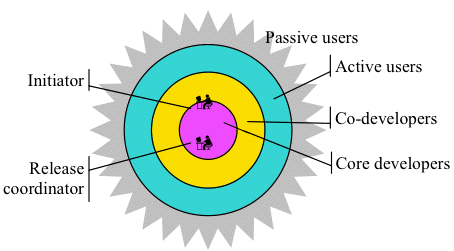
\includegraphics[width=0.6\textwidth]{figures/onion_model.png}
    \caption{Onion model of collaboration types in FLOSS projects \cite{crowstonSocialStructureFree2005}.}
    \label{fig:onion1}
\end{figure}

The onion model describes the types of participants in an OSS project as layers. The center represents the small group of core developers responsible for the majority of contributions to the software. They are surrounded by a larger group of co-developers, whose main contributions are usually bug fixes reported by the active users. The passive users are usually the largest in numbers, who do not contribute or report any bugs. Each contributor layer is about one magnitude larger in numbers than the preceding inner layer in a healthy FLOSS project \cite{mockusTwoCaseStudies2002}.

% AUTHOR NAME HARDCODED HERE
El Asir et al. \cite{elasriPeripheryCoreTemporal2017} used a K-means classification to categorize project participants into a similar core-periphery structure (core, gray in-between area, and periphery) based on SNA metrics with a monthly timeframe and analyzed how and why contributors transition between groups. They found that technical contributions like code commits and lines added have a much heavier impact on becoming a core developer as opposed to other activities, such as testing, reviewing, and commenting.

% AUTHOR NAME HARDCODED HERE
A literature review conducted by McClean et al. \cite{mccleanSocialNetworkAnalysis2021} systematically analyzed the state-of-the-art research of 46 scientific papers in the field of FLOSS collaboration networks and categorized them into three groups based on topic: structure, lifecycle, and communication. They conclude that the existence of core-periphery structure in OSS projects is well established in the field, which is also an indicator of a healthy FLOSS software. Regarding the lifecycle, generally, the core development team does not change significantly over time; however, the project becomes more decentralized and distributed as it matures. A lack of research regarding temporal analyses was identified in the most current knowledge, which is suggested as a future research area in this field.

It is also unknown what practices are followed in OSS development processes, and how closely they are adhering to these practices. It has already been found that the semantic versioning of OSS software does not follow strictly the definition of major-minor-patch releases, with many packages getting stuck at 0 major version, which are still used by other projects as dependencies despite the 0.y.z usually signaling an incomplete software \cite{decanLostZeroSpace2021}. The frequency and regularity of new releases, and what organizational best practices are followed, are also not known.

\subsection{Collaboration network of Open-source projects}
In a larger FLOSS project, developers usually cannot understand every part of the project; therefore, collaboration is required with each other. The graph created by the contributors' interaction can be considered as a network depicting the developers' cooperation and collaboration. Social network theory describes how interaction patterns affect individual behavior \cite{martinez-torresGeneticSearchPatterns2012}. We can model an OSS project's collaboration network as a graph $G(N, E)$, where nodes $N$ represent collaborators (developers, bug reporters, etc\dots) and edges $E$ represent an interaction between them. 

The type of social interaction determines the created network; therefore, choosing the basis of collaboration can significantly impact the network structure. The common types of developer collaboration networks (DCNs) are Version Control System-based (VCS-DCN), Bug Tracking System-based (BTS-DCN) networks, and DCNs, which are purely based on social elements \cite{aljemabiEmpiricalStudyEvolution2018}. The VCS-DCN takes the version control application as a source for network generation by recording collaboration based on co-edits of the same module, file, or code section. Choosing the granularity can impact the precision of true collaborations represented in the network. Co-edits by multiple developers to a single module or file does not necessarily mean actual collaboration was required from the authors, as the parts edited could work functionally independently of each other. By increasing the granularity to file sections (classes or functions within a single file) or even lines, we can be more confident that coordination was required, but we risk leaving out semantically connected parts of the project \cite{joblinEvolutionaryTrendsDeveloper2017}.

In contrast to VCS-DCNs' purely technical approach, the BTS-DCNs use semi-technical bases for connecting participants, such as comments on issues, bugs, or reviews \cite{elasriPeripheryCoreTemporal2017}. Although being tightly related to specific sections of the source code, these artifacts allow for taking into account conversational elements as a contribution. For example, participants, who do not contribute directly to the software source code, but actively review and comment, are also considered. Lastly, networks of developers can be constructed on project participation, following, starring, or through communication means like mailing lists. The technical aspect of collaboration is minimized in such DCNs, and they are more fit for project organization and communication analyses in FLOSS projects.

\subsection{OSS project evolution and success}
Proposed by Lin et al. \cite{linBlogCommunityDiscovery2007} and adopted to the open-source community by Aljemabi and Wang \cite{aljemabiEmpiricalStudyEvolution2018}, five evolution patterns can occur during an OSS project's lifecycle: extinct, emerge, merge, split, and derivation. Extinction occurs when no community members are left to support the project due to joining other DCNs or simply leaving. Emergence happens when a new area of interest has been discovered, attracting new developers to work on the common issue. The merge of two developer networks occurs when two distinct communities come across a similar problem, and their interests align, so they start sharing resources. Split is the reverse process of merging and happens when a community is divided on an issue or bug, creating separate forks and ultimately new communities around the different forks. Derivation is a significant change in the network lifecycle, such as a sudden increase or decrease in size, which can signify a major event in the project.

Therefore, successful projects must create a community structure in which members can efficiently resolve conflicts. Otherwise, the reason why the community emerged is lost from sight, and merges, splits, and even extinction can occur. To maintain a proper focus on the solution the software provides, successful projects use a modular structure after reaching a certain size which ensures that the pieces of the growing software project are kept at a manageable size \cite{antwerpEvolutionOpenSource2010}. Yang et al. \cite{yangHowMicrobloggingNetworks2013} have also shown that digital communication, such as microblogging, plays a crucial role in maintaining a thriving community of both developers and users alike. A successful project (in terms of the number of downloads and commits) tends to have an older follower base with a relatively high number of microblog updates and tags count. To safeguard the continued success of an OSS community, the knowledge centralization at a single or a few developers should be avoided. The Truck factor provides an estimate on the number of key contributors whose removal or absence would significantly set back or disrupt the project's success \cite{avelinoNovelApproachEstimating2016}.


\section{Motivation of research problem and research questions}
\label{sec:motivation-rq}
Because there is a high dependency on the community in open-source software projects, by understanding how contributions are included and what patterns emerge, we can gain valuable insight into its current state and its trajectory. As stated before, SNA analysis of OSS has been extensively studied, but there is a lack of research regarding temporal models analyzing the lifecycle of a FLOSS project.

This paper aims to fill in this gap by examining OSS project collaboration networks over time using SNA metrics. More specifically, one part of the research will focus on the evolution of such collaboration networks and comparing and contrasting these networks across a selection of projects, focusing on lifecycle events such as releases and layoff events. The second part will focus on releases within many projects and how it affects the developer collaboration. The research question, which is broken down into subquestions, is as follows:

\begin{quote}
    \textbf{How do major events in the project lifecycle change the collaboration network of the project?}
\end{quote}
\begin{itemize}
    \item \textit{RQ1: Do planned or foreseeable events change the collaboration structure?} Major software version releases can be considered foreseeable events of the project lifecycle, which could affect the developer collaboration. For example, there might be a higher rate of interaction between contributors before a new version is released to clear up the backlog of tasks. However, it is also possible that commit and change rates drop during this time because the focus shifts to stability and testing instead of new features.
    \item \textit{RQ2: How unforeseeable internal or external events affect FLOSS collaboration?} Sudden shocks to the project, such as an announcement of disinterest from significant users of the software, discontinued enterprise support of the project, large-scale global events like the pandemic, or sudden employee layoffs can significantly affect the core and periphery collaborators alike. By analyzing the collaboration network before, during, and after such changes, we might be able to recognize patterns that regularly occur around these events.
\end{itemize}

\subsection{Research methodology}
To find answers to the research questions above, first, we build a repository analyzer tool, which mines collaboration data from FLOSS projects, generates static snapshot collaboration networks at each given time interval, and calculates SNA metrics for each snapshot. Then these metrics can be aggregated over time or plotted against time to discover changes in the network. The \texttt{git2net}\footnote{\url{https://github.com/gotec/git2net}} \cite{goteAnalysingTimeStampedCoEditing2019} Python library provides the necessary tools to mine any project repository that uses git version control. It also incorporates temporal network generation capability, which can be used to create static collaboration networks aggregated over a given period of time.


We apply a hybrid methodology of qualitative and quantitative research. First, as part of the qualitative research, we choose a small number of repositories to be analyzed. We observe the number of connected components, centrality, number of nodes, and mean degree SNA metrics in order to discover the core and peripheral collaborators over the project lifecycles and observe trends over time. The basis of collaboration, due to the unavailability of other means of communication, is co-editing files. Based on the state-of-the-art research in this field, file co-editing proves to be an effective and easy way to represent collaboration between developers.

After discovering the collaboration structure over time, we will match the breakpoints and unexpected spikes or troughs to events within the project's lifespan. We expect that the key SNA metrics will show a periodicity around planned releases and other reoccurring events (e.g., holiday season). On the other hand, outstanding values without reoccurrence are more likely to be consequences of unexpected events. In these cases, it should be observed whether the network is capable of reorganizing itself or does the event leave a permanent mark on the collaboration structure. A categorization of unexpected events and the level of impact each category has should be observed.

In the quantitative research section, we gather a large set of randomly selected repositories along with the version numbers over time, and we analyze the changes in network statistics at the time of releases, which we interpret with the gained insight during the first, qualitative section of the research.


\section{Gitminer implementation}
\label{sec:gitminer}
To find answers to the research questions, we implement an analysis tool to mine and analyze project repositories, which allows us to generate collaboration networks and network metrics for the analyzed projects.

\subsection{\texttt{git2net} miner}
The process begins with project mining. After cloning the repository, the  \texttt{git2net} \cite{goteAnalysingTimeStampedCoEditing2019} library is used to collect data related to commits. Specifically, who is the author of each commit, which files were modified (created, edited, deleted) with the commit, and when was the commit created. Additionally, the lines edited by the author within each commit are collected separately, allowing for a more fine-grained collaboration network generation if necessary. The results are collected into an \texttt{SQLite} \footnote{\url{https://www.sqlite.org/index.html}} database file's \textit{commits} and \textit{edits} tables.

The \texttt{git2net} mining process by default collects all the commits throughout the project's lifecycle. However, the processing time of each commit differs based on the number of edits, the affected number of files, and the file types as well, which makes collecting specific commits very resource-intense and time-costly. Therefore, we exclude every commit containing more than 100 file modifications during each repository mining using the \textit{max\_modifications} parameter. As observed by Gote et al. \cite{goteAnalysingTimeStampedCoEditing2019}, these exclusion criteria do not significantly affect the generated network because they are mostly merge commits or project restructurings, which do not mark any actual collaboration effort between developers. During the data mining in specific repositories, we encountered commits that were not minable with this method, and the mining process halted, presumably due to processing error because of binary file changes in these commits. We also excluded these commits from our data mining process.

These exclusion criteria resulted in an average of 3\% of commits excluded in all repositories subject to our analyses, with the highest excluded commit rate being 20\%.

\subsection{\texttt{repo\_tools} miner} 

We use the \texttt{repo\_tools} \footnote{\url{https://github.com/wschuell/repo\_tools/}} Python library to query the GitHub API for additional repository data extraction, such as:

\begin{itemize}
    \item Releases
    \item Tags
    \item Issues
    \item Stars and followers
\end{itemize}

The mining output is also stored in an \texttt{SQLite} relational database queried later on during the analysis. 

% - what do we want to achieve with the gitminer
%  - generate networks of collaboration
%    - what should be the basis of collaboration
%  - filter for time
%  - generate statistics

\subsection{Data preprocessing}

The collaboration networks with the \texttt{git2net} library connect the authors to their edited files using only file and author names instead of IDs. This creates an issue when generating the networks because authors with the same name will show up as one node, and they will be connected to the files they touched combined. Furthermore, authors that change their displayed name ('author\_name' field in the mining database) or log in from different accounts, where they have different names, will show up as multiple nodes instead of a single vertex.

We utilize the \texttt{gambit} \cite{goteGambitOpenSource2021} rule-based disambiguation tool to resolve the author names. Furthermore, the created networks have issues when the node names contain special characters or spaces. Therefore, after disambiguation, we replace every unique author name with its ID number.

As the files are also labeled by their filename property in the network outputs, the same filenames in different folders are also displayed as single nodes. In order not to create false collaborations, we remove the files from the network with filenames that occur more than once in all the repository subdirectories. We argue that this does not remove any significant collaboration data since most files sharing their name with other files are technically files, like \texttt{\_\_init\_\_.py} for a Python project.

\subsection{Collaboration networks}

When creating a DCN from the mined data, we have multiple methods at hand. The \texttt{git2net} library provides its own co-editing network function, which returns a temporal network of collaborators. This uses the co-authorship algorithm developed by Gote et al. \cite{goteAnalysingTimeStampedCoEditing2019}; however, we would like to have more control over the network generation method, such as simple file-based co-authorship to customize the network for our needs, like weighing each relation or generating undirected graphs.

\subsubsection{Temporal bipartite network}
As a first step, we generate a temporal bipartite network of authors and their edited files with the \texttt{git2net} built-in \textit{get\_bipartite\_network} method. A temporal network is a \texttt{pathpy} \footnote{\url{https://www.pathpy.net/}} graph object, which contains a collection of timestamped graphs of a single network at each point in time within the observed timeframe. Such a snapshot $S_t = (U, V, E_t)$, where $U$ is the set of authors, $V$ is the set of files, and $E_t$ is the set of file edits as edges at $t$ timestamp. By connecting the authors, who touched the same files, and removing the nodes representing the edited files (converting the bipartite network to a regular network), we can observe the evolution of the collaboration over time, represented in Figure \ref{fig:temporal net}.

\begin{figure}[!htbp]
    \centering
    \begin{subfigure}{0.3\textwidth}
        \centering
        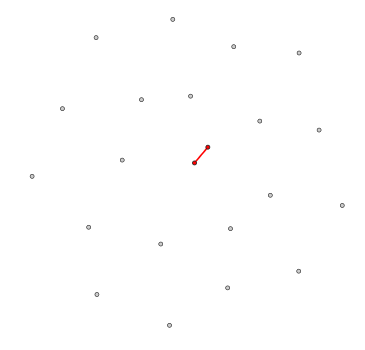
\includegraphics[width=0.92\textwidth]{figures/temporal/0.png}
        \caption{}
        \label{fig:temporal net A}
    \end{subfigure}
    \hfill
    \begin{subfigure}{0.3\textwidth}
        \centering
        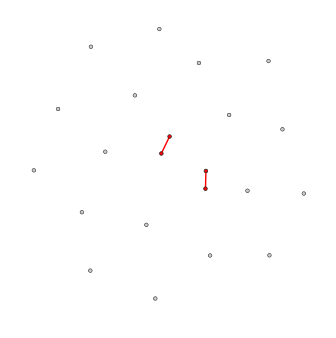
\includegraphics[width=0.92\textwidth]{figures/temporal/1.png}
        \caption{}
        \label{fig:temporal net B}
    \end{subfigure}
    \hfill
    \begin{subfigure}{0.3\textwidth}
        \centering
        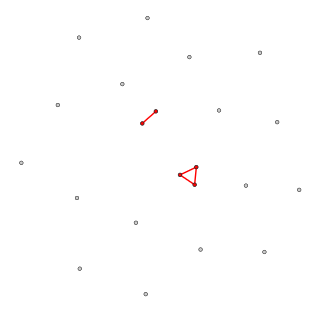
\includegraphics[width=0.92\textwidth]{figures/temporal/2.png}
        \caption{}
        \label{fig:temporal net C}
    \end{subfigure}
    \hfill
    \begin{subfigure}{0.3\textwidth}
        \centering
        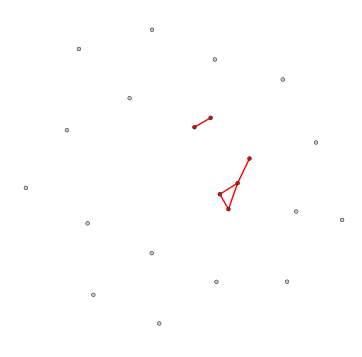
\includegraphics[width=0.92\textwidth]{figures/temporal/3.png}
        \caption{}
        \label{fig:temporal net D}
    \end{subfigure}
    \hfill
    \begin{subfigure}{0.3\textwidth}
        \centering
        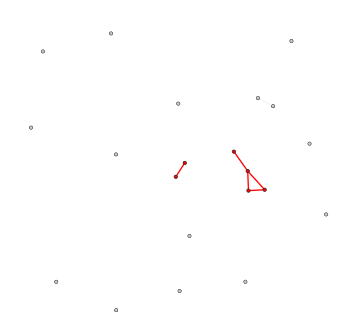
\includegraphics[width=0.92\textwidth]{figures/temporal/4.png}
        \caption{}
        \label{fig:temporal net E}
    \end{subfigure}
    \hfill
    \begin{subfigure}{0.3\textwidth}
        \centering
        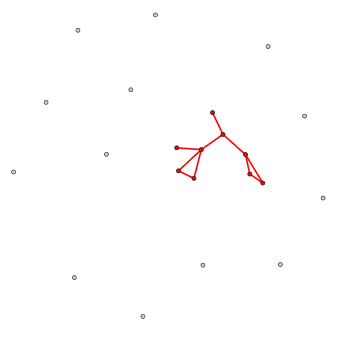
\includegraphics[width=0.92\textwidth]{figures/temporal/5.png}
        \caption{}
        \label{fig:temporal net F}
    \end{subfigure}
    \caption{Sequential snapshots of the \texttt{NetworkX} collaboration network with a moving time-window of 30 days and 7-day steps.}
    \label{fig:temporal net}
\end{figure}

Although a temporal network preserves the time aspect of the graph by the edges being tied to the time dimension of the graph, calculating network metrics like centrality on such networks is infeasible. Visualization also proves to be problematic in representations where animation is not possible. Therefore, we aggregate the bipartite network over a given timeframe into a static network. All nodes within the temporal net are preserved, and all directed edges are added to the network with the edge weight representing how many times that author edited the file.

\subsubsection{Static networks}
The generated static weighted bipartite network loses its time-varying component, but now we can manipulate and calculate complex statistics over it. Figure \ref{fig:bipartite} is an example of such a network. As a next step, we convert the bipartite network into an authors' network by removing the nodes representing files.

\begin{figure}[!htbp]
    \centering
    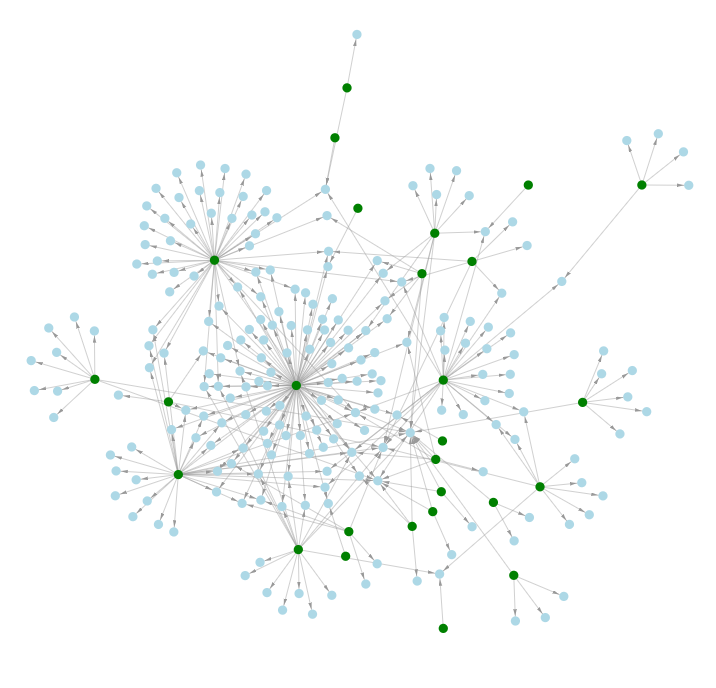
\includegraphics[width=0.65\textwidth]{figures/bipartite.png}
    \caption{A bipartite network of authors (green) and edited files (light blue) in the \texttt{pandas} project within the timeframe 31/01/2021 and 15/02/2021.}
    \label{fig:bipartite}
\end{figure}

We have multiple methods to convert the directed and weighted bipartite network into a projection of authors. We could simply remove the files and connect each author that worked on the same file; however, the result would be an unweighted graph. This would falsely show that all collaborations are weighted equally, which is clearly not the case, as multiple continuous edits on the same file from both parties should represent a stronger collaborative connection. Therefore, firstly we implement the Weighted One-Mode Projection (WOMP) method \cite{stramWeightedOneMode2017}. The WOMP method converts the bipartite network $G(A,F,E)$, where $E$ is the edge list containing tuples $(a_i,f_i,w_{ij})$, and $w_{ij} \in E$ is the weight between author $a_i \in A$ and file $f_i \in F$. With this notation, a weighted directed edge can be calculated for any $a_a, a_b \in A$ as follows:

\[ w_{ab}^{A \rightarrow A} = \sum_{j=1}^m \frac{w_{aj}}{W_a^F}, \]

where $W_a^F$ is the sum of all outgoing edge weights from author $a$ to all files $F$ denoted as $W_a^F = \sum_{i=1}^n w_{ai}$. This creates a bidirectional weighted collaboration network between authors $a_1$ and $a_2$, where the weight $w_{12}$ represents the relative collaboration effort of $a_1$ towards $a_2$ compared to all the other developers $a_1$ has collaborated with. Consequently, every edge is in the range $[0,1]$ in the resulting WOMP network.


A disadvantage of the WOMP method is that the generated collaboration network is bidirectional, meaning if there were any commonly authored files between $a_1$ and $a_2$, then there will be both $w_{12}$ and $w_{21}$ connecting them. To simplify the network, we want to generate an authors network, where the edges are undirected. For this, we are using the weighted Jaccard method on the files-authors bipartite network:

\[ w_{ab} = \frac{\sum_{f \in F}min(f_a, f_b)}{\sum_{f \in F}max(f_a, f_b)}. \]

\begin{figure}[!htbp]
    \centering
    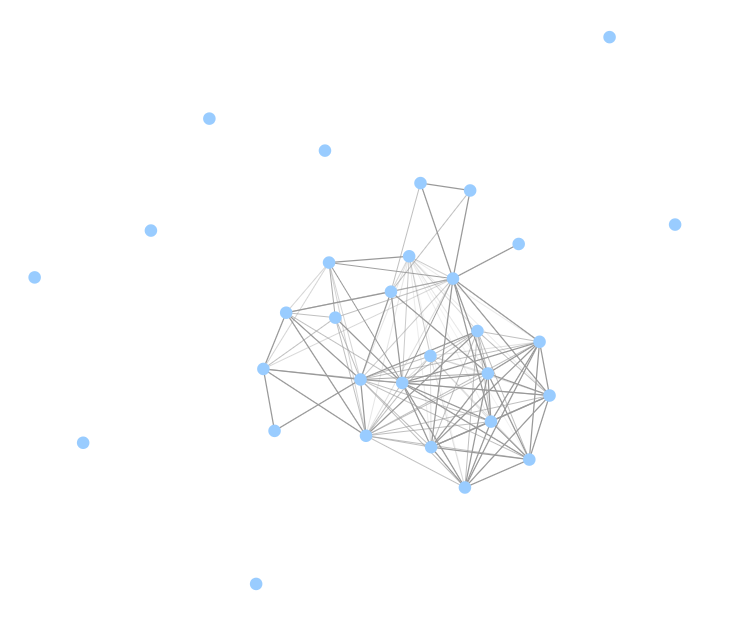
\includegraphics[width=0.9\textwidth]{figures/jaccard.png}
    \caption{Weighted Jaccard similarity collaboration network of \texttt{pandas} generated from the bipartite network in Figure \ref{fig:bipartite} showing the weighted edges within the network.}
    \label{fig:jaccard}
\end{figure}

For each file $f$ that $a_1$ and $a_2$ authors touch, we sum up the minimum and maximum weights the authors have towards each file, and then we divide the sum of minimums with the sum of maximums. This results in the undirected author-author network with edge weights in the range $[0, 1]$. By default, this method removes isolated contributors who do not collaborate with each other but actively edit the files. We add these nodes manually. Figure \ref{fig:jaccard} shows the final author network.


\subsection{Core and periphery, centralization}
A critical part of the OSS software projects is the existence of core and periphery developers. It has been observed that in each FLOSS project, there are a small number of developers who provide the vast majority of development effort into the project. According to the state-of-the-art literature, the members of core developers do not change substantially during the project's lifecycle. However, there was no effort on whether there is a change in the collaboration pattern, especially before, during, or after a significant lifecycle event. Therefore, we make efforts to identify the core developer network to observe these changes.

\subsubsection{Degree centrality}
\label{sec:deg_centrality}

We use the degree centrality of each node (i.e., developer) to identify the core members. The degree centrality of a node is the fraction of all possible nodes it is connected to. We can calculate it by dividing the degree with $n-1$, where $n = |G|$ the number of nodes within the network. Since the core developers contribute the majority of commits and edits of the project, they are expected to be connected with more nodes. Joblin et al. \cite{joblinClassifyingDevelopersCore2016, joblinEvolutionaryTrendsDeveloper2017} have also identified degree centrality as the best predictor of core developers. When binary classification of core or periphery is needed, we assign developers to the core network if their degree centrality score is in the top 20th percentile; otherwise, they are considered periphery. We also note that this method does not consider the weighted edges, only the number of edges (degree) a node has. Although this method could be refined to consider the node degree weighted with the edges, we argue that this could lead to invalidity. In case of two developers, who only contributed to one file, they will be represented with a strong connection and would receive a high weighted degree value, whereas a core contributor, who edits many files, can have many weak connections, but these might not add up to one strong connection of the two isolated developers when weighted with the edge weights. It is clear that a developer with many connections, regardless of the strength of the collaboration, should be considered core. Figure \ref{fig:degree centrality} shows two examples for degree centrality within a collaboration network. In the figure, darker colors represent a higher degree centrality value. The highlighted nodes are in the highest 20th percentile of degree centrality, classifying them as members of the core developers. We can observe that \texttt{pandas} is much more decentralized in both one-month periods, whereas \texttt{curl} is mainly dependent on one developer.

\begin{figure}[!htbp]
    \centering
    \begin{subfigure}{0.49\textwidth}
        \centering
        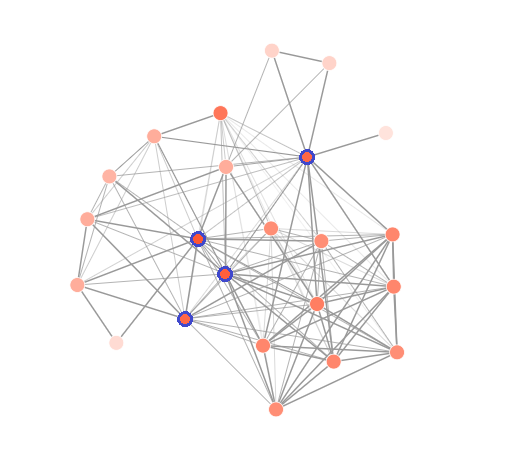
\includegraphics[width=0.98\textwidth]{figures/degree_centrality.png}
        \caption{Pandas}
        \label{fig:centrality a}
    \end{subfigure}
    \hfill
    \begin{subfigure}{0.49\textwidth}
        \centering
        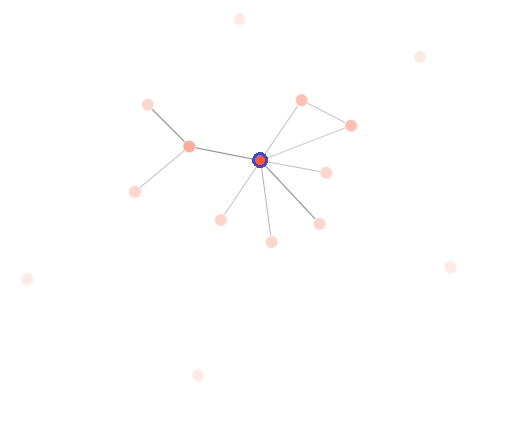
\includegraphics[width=0.98\textwidth]{figures/degree_centrality_curl.png}
        \caption{Curl}
        \label{fig:centrality b}
    \end{subfigure}
    \caption{Degree centrality within the \texttt{pandas} and \texttt{curl} projects' collaboration networks, showcasing a decentralized (a) and heavily centralized (b) network as examples.}
    \label{fig:degree centrality}
\end{figure}

\subsubsection{Degree centralization}

The degree \textit{centrality} can be calculated for every node, but through our analysis, we would also like to measure a global \textit{centralization} metric, which is applicable to the whole network. As suggested by Crowston and Howison \cite{crowstonHierarchyCentralizationFree2006}, we calculate the degree \textit{centralization} by summing the differences between the maximum and each node's degree \textit{centrality}. 

\[ C_D(A) = \frac{\sum_{i=1}^n(C_d(a*)-C_d(a_i))}{H}, \]

where $C_d(a)$ is the degree \textit{centrality} of an author $a$, $a*$ is the author with the highest degree \textit{centrality} value, and $n$ is the number of authors in the collaboration network $A$. The value $H$ is for normalizing the sum by dividing by the theoretical maximum \textit{centralization}. Since the \textit{centrality} values are already in the range $[0, 1]$, we only need to normalize for the network's size. We get the highest centrality score with a star graph, where each node is only connected to a single central node, which has precisely one edge to all other nodes. The central node has a centrality of 1 in this case, whereas all the other $n-1$ nodes have $C_d(a) = \frac{1}{n-1}$. This means that in the case of a star graph:

\[ H = (n-1) (1-\frac{1}{n-1}) = n-2. \]

When a project is inactive within certain timeframes, it could happen that the network contains two nodes or fewer. We define $C_D(A) = 0$ if $|A| = n <=2$. The resulting output will always have a value in $[0, 1]$, where 1 means a completely centralized network (star graph) and 0 means a completely decentralized network. It is important to emphasize that a centralization score of 0 does not necessarily mean that there is no collaboration and every developer is isolated. Rather it means that each developer is co-authoring with just as many authors as the others do.

% - \cite{klugUnderstandingGroupDynamics}

\subsubsection{Clustering coefficient}
\label{sec:clustering}

\begin{figure}[!htbp]
    \centering
    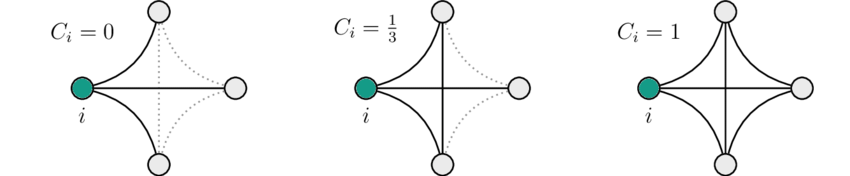
\includegraphics[width=1\textwidth]{figures/loc_clust_coeff.png}
    \caption{The local clustering coefficient demonstrated on an unweighted network of 4 vertices \cite{jedrzejewskiRoleComplexNetworks2016}.}
    \label{fig:loc clust coeff}
\end{figure}

While centralization helps us describe the centralness of the network and how much it is centered around a single or a few developers, it does not help us describe the structure of the network in more detail. Our goal is to gain an understanding of also the modularity of our network, meaning how much developers tend to cluster together \cite{joblinEvolutionaryTrendsDeveloper2017}. We expect that authors form smaller clusters, which are more tightly connected, and these clusters have somewhat weaker ties to other clusters. This builds on the assumption that the collaboration network of the software follows the modules which build up the software itself, thus authors of a specific function should also cluster together within the network \cite{conwayHowCommitteesInvent1968, joblinEvolutionaryTrendsDeveloper2017}. To measure this 'clusteredness', we calculate the \textit{local clustering coefficient} for each node.

The \textit{local clustering coefficient} quantifies on a scale $[0, 1]$ how likely it is that a node's neighbors are also neighbors. We use the number of triangles (also called clique, triplet) between neighbors the node is a part of. This is illustrated for unweighted networks in Figure \ref{fig:loc clust coeff} with the formula:

\[ C_i = \frac{2T(i)}{deg(i)(deg(i)-1)}, \]

where $T(i)$ is the number of triangles through node $i$ and $deg(i)$ is the degree of i. However, in a weighted network, we also have to consider the edge weights since it is easy to see that a clustering coefficient of 1 with also the top-weighted edges in a triplet does not represent the same clustering as being connected with a weak link. We expect weaker links connecting larger clusters, whereas stronger links within each cluster. Therefore, we use geometric averaging of the subgraph edge weights (as implemented by the \texttt{NetworkX}\footnote{\url{https://networkx.org/documentation/stable/reference/algorithms/generated/networkx.algorithms.cluster.clustering.html}} library \cite{onnelaIntensityCoherenceMotifs2005}):

\[ c_i = \frac{\sum_{jk}(\hat{w}_{ij}\hat{w}_{ik}\hat{w}_{jk})^{1/3}}{deg(i)(deg(i)-1)}. \]

The $\hat{w}_{ij}$ represents the normalized weight of edge $e_{ij}$ over the maximum weight in the network.

\subsubsection{Hierarchy}
\label{sec:hierarchy}

The degree centrality and the clustering coefficient are in themselves able to express meaningful aspects of the developer collaboration network; however, by combining the two metrics, we can also assess how hierarchical the network is. In a scale-free hierarchical network (such as the collaboration network), nodes tend to cluster around a single or a few hubs, which are more likely to have weak connections to other hubs \cite{ravaszHierarchicalOrganizationComplex2003, joblinEvolutionaryTrendsDeveloper2017}. The nodes within these formed groups are relatively stronger than the connections connecting the hubs, but they are less likely to connect to nodes outside their group. Therefore, in a hierarchical network, the hubs have a high degree number and a low clustering coefficient, whereas the group members clustering around the hubs have a high clustering coefficient but low degree numbers.

We can visualize the degree of hierarchy by plotting each node's clustering coefficient against the number of degrees, shown in Figure \ref{fig:hierarchy}. The plotted linear regression trendline will decrease steeply in hierarchical networks, as there is a negative correlation between the degree and clustering coefficient. In networks where this cannot be observed, the trendline stays flat, meaning these two metrics are independent of each other, and the structure is not hierarchical. To measure the hierarchical level numerically within a network, we take the trendline's slope, which is $\beta_1$ in the $y=\beta_1x + \beta_0$ general linear regression equation.

\begin{figure}[!htbp]
    \centering
    \begin{subfigure}{0.49\textwidth}
        \centering
        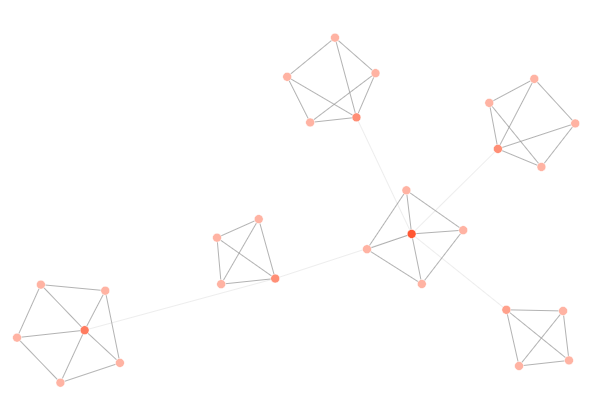
\includegraphics[width=0.98\textwidth]{figures/hierarchical.png}
        \caption{Highly hierarchical network}
        \label{fig:hierarchical}
    \end{subfigure}
    \hfill
    \begin{subfigure}{0.49\textwidth}
        \centering
        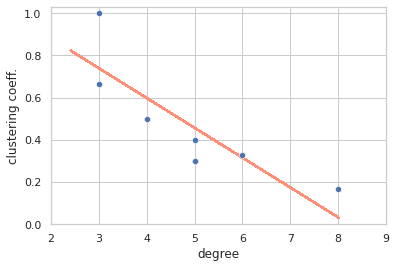
\includegraphics[width=0.98\textwidth]{figures/hierarchy_plot2.png}
        \caption{Network hierarchy}
        \label{fig:hierarchy plot}
    \end{subfigure}
    \caption{Hierarchical network and its corresponding degree number vs clustering coefficient plot.}
    \label{fig:hierarchy}
\end{figure}

In every network, isolated authors can be observed who are only working on files that no one else has edited (in the given timeframe). These nodes can skew the hierarchy score because an isolated node's degree and clustering coefficient are by definition 0, which disproportionately makes the trendline much flatter. Therefore, we remove the isolated nodes from the network. If the network only contains isolated nodes, and there is no linear regression to be calculated, we set the hierarchy value to 0.

\subsection{Project measures}

One of our assumptions is that the collaboration network structure changes depending on the project's lifecycle. In order to discover cause and effect relationships between the network structure and project lifecycle, we gather basic project metrics to pinpoint the time and date of events, as well as the effort required within the project. We achieve this by gathering the dates of each release, and the quality and relative stress is measured by the issues within the project (create and close times).

\subsubsection{Release and release measures}

To measure the network changes around releases, we first collect the list of releases for the given project. Our goal is to gather the version number of each release, as well as the dates they were released. There are two relevant APIs regarding the release version numbers: GitHub releases and Git tags. Tags are marked and annotated commits supported by Git, therefore other projects that are not on GitHub can also have tags. \textit{Tags} are most commonly used to mark new release versions, but they can also be used to annotate other information, such as release editions or milestones. On the other hand, a \textit{Release} is a high-level GitHub concept, which allows the project organizers to announce Git tags as project releases by adding a version number, release notes, and binary artifacts \cite{olsonReleaseYourSoftware2013}. A commit that represents a new GitHub release must be tagged, but a tagged commit does not necessarily need to be a new GitHub release.

Throughout our analysis, we use the tags as indicators of a new release, because there could be new versions of a software that are not released publicly and therefore do not have a GitHub release. Furthermore, GitHub only announced the Releases workflow in 2013, when the release versioning by Git tags was already a common practice. This means that releases before 2013 can only be analyzed via the repository tags.

Most large-scale OSS projects follow the semantic versioning convention, but only to a certain extent. The majority of tags follow the major-minor-patch (also known as breaking-feature-fix) semantic version naming convention in the format of X.Y.Z, where X is the major number, Y is the minor number, and Z is the patch number \cite{preston-wernerSemanticVersioning}. At the end, optionally, pre-release and build data can be marked, for example, \textit{1.11.6-pre}. The major number signifies an API-breaking change compared to the previous release, meaning backward compatibility is not guaranteed for depending applications. Minor releases add new features, but compatibility is ensured with the older version. Patch releases usually handle bugs and security updates within the package.

\begin{figure}[!htbp]
    \centering
    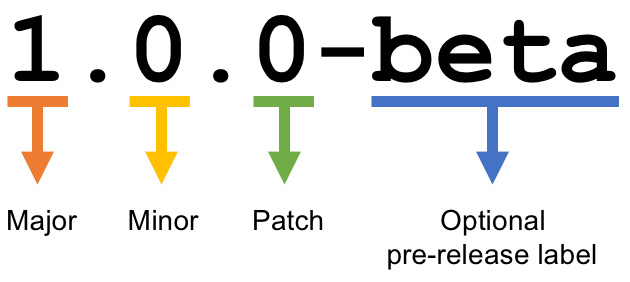
\includegraphics[width=0.5\textwidth]{figures/semantic-versioning.png}
    \caption{Semantic versioning illustrated. Figure source: \cite{mariogripSemanticVersioningUT2018}.}
    \label{fig:semver}
\end{figure}

During the network analysis, we expect the network measures to change around a release, but it is also expected that a larger release requiring more collaboration will have a more significant impact, while smaller changes have minor or no impact at all. The issue with the semantic versioning and release names is that there are no constraints, which would enforce a strict version naming, and it is entirely up to the developers to set the tag names. This leads to inconveniences when measuring collaboration effort through release version number because a patch might require more collaboration effort than a minor release, and a minor release within one project could require significantly more teamwork than in another. Furthermore, tag names can be inconsistent, and there could be version numbers that do not adhere to the major-minor-patch naming convention at all (e.g., test releases, or releases like 'latest-release-v11'). The possibility to add extra information at the end of tag names, like \texttt{-beta} or \texttt{rc}, further complicates tracking the collaboration effort because the majority of collaboration effort might happen before the \texttt{rc} version, or it might happen after it. As it can also be seen in Table \ref{tab:releases}, the \texttt{v0.14.0rc1} tag contains more modifications than the final \texttt{v0.14.0} version, whereas the \texttt{v1.2.0rc0} only contains a small fraction of modifications compared to \texttt{v1.2.0}.

\begin{table}[!htbp]
    \centering
    \resizebox{\textwidth}{!}{%
        \begin{tabular}{| c | c | c | c | c | c | c | c | c |}
            \hline
            \textbf{Index} & \textbf{Name} & \textbf{Tag name} & \textbf{Created} & \textbf{Type} & \textbf{Modifications} & \textbf{Lines added} & \textbf{Lines removed} & \textbf{Total change} \\
            \hline \hline
            0 & Pandas v0.13.0 & v0.13.0 & 2013-12-30 17:02:51 & unknown & 20031 & 1.665357e+09 & 1.624343e+09 & 3.289700e+09 \\
            1 & Pandas v0.13.1 & v0.13.1 & 2014-02-03 04:52:01 & patch & 836 & 2.231875e+06 & 2.349833e+06 & 4.581708e+06 \\
            2 & Pandas v0.14rc1 & v0.14.0rc1 & 2014-05-16 22:28:09 & minor & 1861 & 2.251189e+07 & 2.050846e+07 & 4.302035e+07 \\
            3 & v0.14.0 final & v0.14.0 & 2014-05-30 11:47:40 & unknown & 318 & 3.220804e+06 & 5.314470e+05 & 3.752251e+06 \\
            4 & v0.14.1 final & v0.14.1 & 2014-07-10 23:46:19 & patch & 720 & 1.660133e+06 & 3.796690e+05 & 2.039802e+06 \\
            5 & v0.15.0 Pre-release & v0.15pre & 2014-09-07 12:52:01 & unknown & 826 & 1.028779e+07 & 2.458664e+06 & 1.274645e+07 \\
            \dots & \dots & \dots & \dots & \dots & \dots & \dots & \dots & \dots\\
            66 & Pandas 1.1.5 & v1.1.5 & 2020-12-07 11:42:10 & patch & 2167 & 4.251057e+06 & 4.611365e+06 & 8.862422e+06 \\
            67 & Pandas 1.2.0rc0 & v1.2.0rc0 & 2020-12-08 12:31:44 & minor & 41 & 1.060500e+04 & 8.850000e+02 & 1.149000e+04 \\
            68 & Pandas 1.2.0 & v1.2.0 & 2020-12-26 13:47:00 & unknown & 683 & 5.782570e+05 & 2.989310e+05 & 8.771880e+05 \\
            69 & Pandas 1.2.1 & v1.2.1 & 2021-01-20 11:21:02 & patch & 1306 & 1.864636e+07 & 9.228629e+07 & 1.109326e+08 \\
            70 & Pandas 1.2.2 & v1.2.2 & 2021-02-09 10:55:19 & patch & 844 & 6.783283e+06 & 1.827142e+07 & 2.505470e+07 \\
            71 & Pandas 1.2.3 & v1.2.3 & 2021-03-02 09:43:36 & patch & 959 & 1.002189e+07 & 5.783745e+06 & 1.580563e+07\\
            72 & Pandas 1.2.4 & v1.2.4 & 2021-04-12 15:59:13 & patch & 289 & 3.402820e+05 & 1.704960e+05 & 5.107780e+05\\
            \hline
        \end{tabular}} \\
    \caption{Releases collected information.}
    \label{tab:releases}
\end{table}

In order to have a more fine-grained measure of how much effort a release required (besides the semantic versioning), we measure the number of lines added and lines removed in that release. This is calculated by adding up each commit's 'total lines added' and 'total lines removed', which was authored after the previous release but up to and including the current release tag's commit. The total change of lines for a release is simply the sum of lines added and lines removed, which are provided by the \texttt{git2net} miner. The miner also provides the number of modifications for each commit. A modification is a section of the source code modified, which can mean multiple lines added and deleted at the same part of the document. For example, if a new function is added to the project, which requires 20 new lines and removes two lines (e.g., empty space that was there before), then it will be considered as one modification, but 22 total line change. Changes to binary files are due to generated artifacts, which do not carry any collaboration effort; therefore, they are excluded, and commits that do not have a hash are also removed.

The release type contains the semantic version of the release, which was gathered from the tag name with a Regular Expression matching the conventional versioning X.Y.Z. We also capture the version number in tags that contain additional notations such as \texttt{beta} or \texttt{rc}; then, we compare the current release to the previous to identify whether the release is a major, minor, or patch release. When the found version numbers in the previous and the current release are the same, we leave that as unknown, as this is mostly the case in pre-releases. The first release does not have a preceding tag; therefore, we consider every modification before the tag as part of the release. This leads to the first tag seeming to have significantly more edits than the rest of the releases, whereas this is just the result of not tracking from the beginning (see example in Table \ref{tab:releases}). Therefore, in our analyses, we remove the first release, as this would lead to falsely weighing the network results.



\subsubsection{Project issues and measures}
\label{sec:project_issues}

To measure the productivity within the project, we collect some basic information regarding the GitHub issues. Issues keep track of bugs, features and tasks, contributors can comment and discuss the task at hand within an issue, and it can be assigned to users, and milestones can be set. We collect the following information of issues:

\begin{itemize}
    \item Issue title
    \item Issue number
    \item Created at
    \item Closed at
    \item Open for
    \item Bug or feature
\end{itemize}

The \textit{issue title} is a short description of the issue. Most projects create their own convention of naming and tagging issues. For example, each issue starts with a 3-letter abbreviation of a category, e.g., \texttt{BUG} or \texttt{DOC}. \textit{Issue number} is a unique number for each issue that is increased sequentially. \textit{Created at} is the date and time of the issue being created, and \textit{closed at} is the time when it was closed. If the issue was still open on the day of data mining (May 9, 2021), this field is empty. The \textit{open for} field is the difference between the \textit{closed at} and \textit{created at} dates, or it is empty if the issue was never closed.

The last measure is \textit{bug or feature}. Because issues can cover a wide range of possible topics, from discussions to performance, it is worth categorizing them to analyze the differences. However, categorization in practice proves to be difficult due to the different conventions each project uses and because GitHub does not apply any constraints to the text of the title. We search for specific keywords in the \textit{issue title} to categorize each issue into either a bug or a feature. We also drop some words from the text because they would give us 'false positive' matches. If keywords for both or neither categories are found, the issue is marked as unknown. The dropped words, as well as the bug and feature keywords, can be seen in Table \ref{tab:keywords} Although this simple method can already classify 10-15 percent of issues, it would require extensive manual effort to improve this ratio further. In future research, sentiment analysis of issue titles and issue descriptions could achieve much higher percentages.

\begin{table}[!htbp]
    \centering
        \begin{tabular}{| c | c | c |}
            \hline
            \textbf{Drop words} & \textbf{Bug keywords} & \textbf{Feature keywords} \\
            \hline \hline
            debug & bug & feature \\
            debugger & defect & enhancement \\
            debugging & incorrect & improvement \\
             & unexpected & suggestion \\
             & error & wishlist \\
             & missing & wish list \\
             & warning & \\
             & problem & \\
            \hline
        \end{tabular}
    \caption{Keywords and drop words for \textit{bug} and \textit{feature} categorization.}
    \label{tab:keywords}
\end{table}

Statistics for issues like average close time also prove to be difficult because there are continuously open issues, which inevitably leads to the fact that a large portion of issues was still open and continues to be open. We cannot know the issue close time for these issues, and if we try to calculate global measures by aggregating all (or portion) of issues, we have to consider the \textit{survival bias} \cite{jarczykSurgicalTeamsGitHub2018}. Figure \ref{fig:survival} shows the issues survival curve of the \texttt{pandas} library. It is clearly visible that a large portion (20 percent) of issues are not closed, and if we left them out of aggregate values such as average open time, our data would be skewed. Nevertheless, we can see in the example that the categorization of issues makes a difference, as bugs get closed a bit earlier than an average (unknown) issue because, after the same amount of days pass for both categories, more bugs tend to be closed in this example. In contrast, features have a high life expectancy, as they are more likely to be still open than a bug if the same number of days pass. The reason could be that features take longer to develop and plan than bugs, which is consistent with the findings of Jarczky et al. \cite{jarczykSurgicalTeamsGitHub2018}.

\begin{figure}[!htbp]
    \centering
    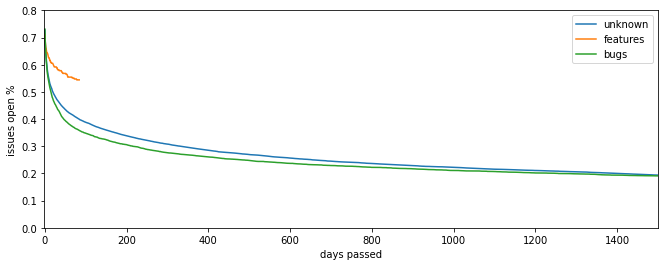
\includegraphics[width=0.9\textwidth]{figures/issues_open.png}
    \caption{Survival curves of the \texttt{pandas} library depicting the slightly lower-than-average lifespan of bug issues, and the relatively long time the features are open.}
    \label{fig:survival}
\end{figure}


\section{Collaboration pattern analysis}
\label{sec:patterns}
The focus of our analysis is how the collaboration network of FLOSS projects changes during their lifecycle. Moreover, we are also interested in the cause of the changes, rather than just observing the changes. Therefore, we determined two types of events that we want to observe to see the effects on the collaboration. The events during a project's lifecycle can be one of two types: regular or irregular events. Regular events repeat over time, with roughly the same time passing between events. This can be a holiday season (e.g., summer holidays or at the end of the year) or regular software releases. Our research focuses on only the software releases, and we suggest the analysis of collaboration and seasonality as a future research topic. In contrast to releases, which are usually well documented and easily discoverable when exactly they were released, irregular events are harder to discover, as these do not necessarily stem from within the developer community but from external sources. Examples could be a supporting company's organizational restructuring, the sudden increase of work from home during the Covid-19 pandemic, or mass layoffs within the support team. In our analysis, we mainly focus on releases, because unexpected events such as layoffs are difficult to collect. The main source for such events are general news sources, which are often based on rumors rather than facts, therefore they can be unreliable. Also, layoffs can have wildly different effects on the collaboration network based on how much the support is being withdrawn, making general conclusions about these events much harder to find. On the other hand, releases can be more easily and reliably collected via git tags and GitHub releases. Our main goal is to observe how the DCN changes before, during and after a release, what patterns emerge and how these observations correlate with the project issues and release frequency.

As a first step, we conduct a qualitative analysis on several hand-picked repositories to observe the network statistics in detail and identify cause and effect relationships. In order to avoid bias when selecting repositories, we choose projects based on a variety of factors:

\begin{itemize}
    \item \textit{Project size:} We define the project's size as small, if it has less than 100 contributors, medium-sized if the number of collaborators is between 100 and 500, and large if it has more than 500 collaborators.
    \item \textit{Centralization:} Although it is hard to measure how decentralized a project is, extensive projects tend to be decentralized based on the literature review. For now, we consider those projects centralized, which have been identified as centralized in the current state-of-the-art literature. 
    \item \textit{Event occurrences:} Whether there is a regular release cycle within the project or not based on the release dates, or if there are known and confirmed cases of unexpected layoff events.
\end{itemize}

Based on these criteria, we try to select a wide variety of projects so that each type (small, medium or large size, centralized or decentralized, regular or irregular or abandoned projects) has at least one example. We acknowledge the fact that these inclusion criteria leave room for selection bias, as an observed correlation between events and the network in one project might not hold true for all projects. However, later we confirm our hypotheses with a quantitative analysis.

\subsection{Project selection and descriptions}

Altogether, we choose eight projects to analyze; these can be seen in Table \ref{tab:projects}. Due to the repository miner's limitation, we are only considering projects maintained on GitHub. The \texttt{pandas} and \texttt{NumPy} repositories are well-known and popular data science tools for data manipulation in Python. They are very similar in size and popularity, both with a considerable base of collaborators. Since the number of issues is also really high, we expect that these projects are highly decentralized, where the developers mainly work on their own parts of the project. They also have pretty regular release cycles, with a minor release every 5-6 months.

\texttt{NetworkX} and \texttt{seaborn} are both middle-sized repositories based on the number of contributors, and they are both used for data visualization and statistical analysis in Python-based software. However, \texttt{NetworkX} visualizes networks and their related statistics, while \texttt{seaborn} creates various plot images. Each release date follows the previous with 4 to 10 months, which means their releases are not as regular as the first two repositories.

The project \texttt{curl} is an example Of a highly centralized project, as its source code is famously maintained by a single developer \cite{crowstonHierarchyCentralizationFree2006}. Based on the number of contributors, it is a medium-sized project, although the number of commits is much higher than \texttt{NetworkX} or \texttt{seaborn}. Being the oldest project from the selection might contribute to the large number of commits.

\begin{table}[!htbp]
    \centering
    \resizebox{0.85\textwidth}{!}{%
        \begin{tabular}{| c | c | c | c | c | c | c |}
            \hline
            \textbf{Name} & \textbf{Contributors} & \textbf{Size} & \textbf{Commits} & \textbf{Stars} & \textbf{Issues} & \textbf{First release}\\
            \hline \hline
            pandas & 2333 & large & 26792 & 29700 & 3518 & Feb 20, 2011 \\
            NumPy & 1135 & large & 26392 & 17200 & 2030 & Jan 5, 2002 \\
            NetworkX & 469 & medium & 6470 & 9100 & 166 & Jul 17, 2005 \\
            seaborn & 140 & medium & 2780 & 8400 & 82 & Oct 28, 2013 \\
            curl & 701 & medium & 27159 & 20600 & 27 & Mar 14, 2000 \\
            servo & 1101 & large & 44084 & 19600 & 3305 & May 22, 2017 \\
            Wasmtime & 243 & medium & 8334 & 5200 & 341 & Oct 18, 2016\\
            py-junos-eznc & 69 & small & 2486 & 583 & 76 & Nov 3, 2013\\
            \hline
        \end{tabular}}
        \caption{Collaboration analysis projects and basic statistics.}
        \label{tab:projects}
\end{table}

\texttt{Servo} and \texttt{Wasmtime} are both based on the Rust programming language, and they are both used for web applications: \texttt{Servo} is a browser engine, whereas \texttt{Wasmtime} is a runtime environment for WebAssembly. Both projects were led by Mozilla and maintained in an open-source environment. The Rust developer team was heavily affected by the Mozilla layoffs on January 15, 2020, and August 11, 2020 \cite{lardinoisMozillaLays70,kastrenakesMozillaLaying2502020}, with the second round of layoffs affecting all Rust employees. The \texttt{py-junos-eznc} project is considered small since it has less than 100 contributors, and it is a Python-based library for automatizing devices running on Juno OS. On May 27, 2020, the sponsoring company Juniper Networks laid off its entire open-source developers \cite{brasseurFarewellJuniperNetworks2020}. These three projects are the main focus of analyzing unexpected, one-time events and layoffs, where we will take a close look at the network statistics around the mentioned dates.

To reliably compare the projects, we have to consider only a slice of each project, so all of them are compared within the same time period. We take a 3-year period from 2018 to the end of 2020. All projects had their first release before this period, which means this should filter out the initial irregular activities, such as creating directories and restructuring.

\subsection{Commits analysis}

For the selected period, we check the number of commits in each project as a first step. This can be seen in Figure \ref{fig:commits}. To smooth out the stacked area plot, we summed up the number of commits every 28 days. Purposefully a multiple of 7 was chosen in order to even out the possible irregularities caused by the weekdays and weekends. We can see that all projects are active, with a varying magnitude of commits generated each month. The number of commits is consistent with the size of the project. However, we can also see that the number of contributors and the number of commits is not entirely dependent on each other, as \texttt{servo} consistently receives more commits than the other large repositories, although it has the same number of contributors as \texttt{NumPy} and half as many as \texttt{pandas}. We assume that this is highly dependent on the type of software being developed, the used programming language(s), and other project-specific properties.

There is a noticeable decrease in the number of commits to \texttt{servo} at the time of the layoffs (August 2020), which signals that the project could have been affected. However, this cannot be observed for \texttt{Wasmtime}. Furthermore, we do not see any evidence of reoccurring trends within the number of commits, e.g., decreased activity during the holiday season. There is a reduction in all repositories at the end of 2018, but a spike contradicts this in the number of commits at the end of 2019. However, we cannot rule out any periodicity because this could be hidden due to the 28-day aggregation.

\begin{figure}[!htbp]
    \centering
    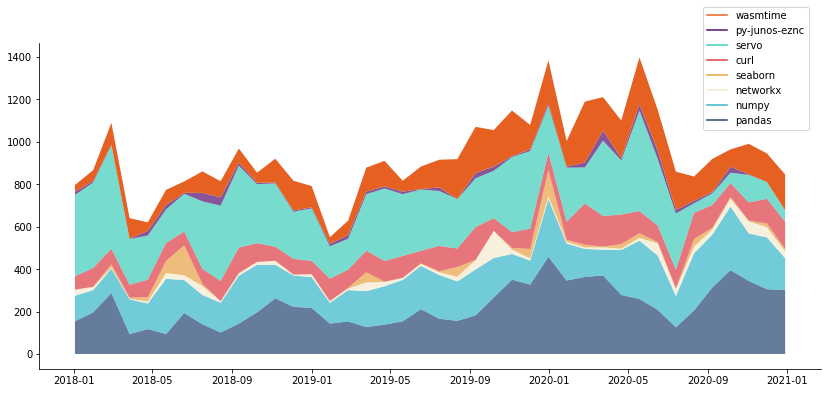
\includegraphics[width=\textwidth]{figures/commits.png}
    \caption{Number of commits in each month.}
    \label{fig:commits}
\end{figure}

\subsection{Releases}
\label{sec:releases}
As a next step, we look at the regular lifecycle events, which are the releases in the open-source projects. We generate the collaboration networks for the same period (between 2018 and 2020) and contrast them with the time of releases.

The issue with generating the collaboration network is the time aspect: we cannot observe any collaboration network if we take a single point in time and create the network for a given timestamp, as this will only contain a handful of connections, who authored an edit in the same file at the exact same time. Therefore, we need to aggregate the edits and commits over time, which requires us to use a time window to scan through the observed time period, and for each step, we generate a snapshot of the network. The first parameter is the time window length, and the second is the step size. By choosing a large time window, we observe more connections within the generated graph, but with a too-large value, the network becomes too much grouped, with almost every node connecting to almost all other nodes. By setting this value too low, the result is a disconnected network. The step size determines how often we take a screenshot of the network for the time window. By default, we use one-day steps, but sometimes this results in too radical changes. Therefore, in some cases, we use a 7-day or a 28-day step value to smooth out the curves. However, a too-high step value can obscure the changes we want to observe.

\subsubsection{Node counts}

First, we take a look at the number of developers in the network over time. The number of nodes (i.e., developers) in the network indicates the activity level within the project, where a relatively high number of nodes imply a peak in project activity, and a low number can imply a decreasing activity, or that the project has become more centralized. It is easy to see that if the only source of activity is one single developer over the observed period, then the network will only have one node, whereas if the same activities are distributed, more developers will be shown in the network, and the number of nodes will rise. However, this does not describe the relationship between developers, they could be completely isolated, or they could be relying a lot on each other regarding collaboration.

In Figure \ref{fig:nnodes} the number of nodes is plotted with the time of releases marked with a vertical black line for each project. The type of release corresponds to the type of line: major releases are shown with a continuous line, minor releases are thick dashed lines, and patch releases are thin dotted lines. The continuous red lines mark an unexpected layoff event, which might affect the project. Each node count data point at $t$ time represents the number of nodes within the collaboration network generated between $t$ and $t+28$ days, with a 7-day step size. The average node counts correlate with the size of the project, as the smaller repositories like \texttt{py-junos-eznc} and \texttt{seaborn} have the number of nodes consistently below 10, while the larger projects can reach 30, 50, or even 100 at specific time periods.

\begin{figure}[!htbp]
    \centering
    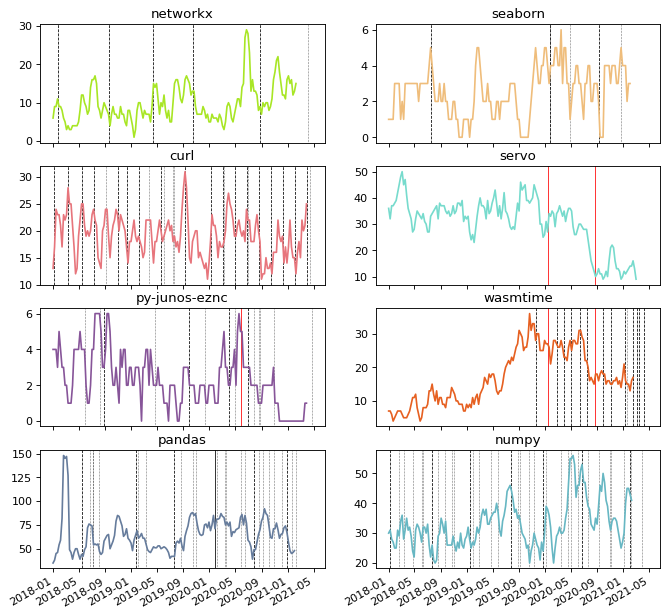
\includegraphics[width=\textwidth]{figures/qualitative/number_of_nodes/all_v2.png}
    \caption{Number of nodes over time.}
    \label{fig:nnodes}
\end{figure}

Regarding the releases, we can see that each project can have a completely different release planning and schedule, making it hard to compare them. Some projects, like \texttt{NetworkX}, \texttt{pandas}, or \texttt{NumPy} release a minor version approximately every six months, while \texttt{curl} does the same every two months. \texttt{Wasmtime}'s release schedule regarding minor releases is even shorter, but we do not have any data available before 2020, which does not allow us to confirm whether this is a long-term trend. The release data for \texttt{servo} was available to us; however, the repository has a very high frequency of releases, with sometimes multiple minor releases in the same week, and displaying this information on the chart would have obscured the number of nodes plot; therefore, we only display the unexpected events. Also, releases can be arbitrarily named by the developers; therefore, a minor release in one project might be considered a patch or a major release in others.

Comparing the events with the number of nodes, we can observe that before or around a minor release, most projects experience an uptick in node count, usually followed by a drop — although not in every case. This can be attributed to the increased activity from the community before the release. There could be several factors causing this activity change: first, if the release date is fixed, the pressure on developers to include the planned features increases, which prompts more activity (pull model). Secondly, the rise in activity could be a newly implemented feature or a recently found bug, which needs immediate attention from developers. In this case, the increased activity and larger volume of edits may prompt a new release version (push model). Our assumption regarding whether a release follows a push or a pull model is that it can be highly dependent on the project, and within each project, there could be a mixture of releases following both models. We cannot observe this trend for the patch releases, and we cannot draw a definitive conclusion regarding major releases, as there was only one major release among all the repositories subject to our analysis.

Regarding the layoff events marked with red vertical lines, a significant drop in the number of nodes can be observed shortly before the event in all projects. After the companies stop supporting the project and lay off the development team, or the team is reassigned to other topics, the number of nodes within the projects drops and stays low, never reaching the same numbers as before. In the case of \texttt{servo} and \texttt{Wasmtime}, the first wave of layoffs does not seem to have a significant impact on the number of nodes. However, we do not have reliable information regarding how much the Rust development team was impacted by the first wave, on which both projects depend.

\subsubsection{Network density and mean degree}
\label{sec:density_degree}
As a next step, we plot the network density and mean degrees of the projects. The network density tells us how densely connected the network is on a scale of $[0,1]$, where one means every node is connected to all other nodes, and 0 means there are no edges in the graph. It refers to the ratio between all the possible connections and the actual connections. Although the generated networks are weighted, we do not consider the edge weight when counting each node's degree, meaning every connection is counted. We expect this value to rise if developers need to reach out to more community members and collaborate on more files with others. Similarly to the density, the mean degree value also only takes the number of nodes (N) and the degree number (k) of each node as inputs, so we expect similar results between the two measures.

By plotting the two measures on the same figure in Figure \ref{fig:density_a}, we can confirm that they are closely correlated. The values are also highly sensitive regarding the number of nodes within the graph, and a low node count makes the graph values change radically. This is why the smaller projects are not shown, as their graph did not convey any meaningful observations. We can identify some troughs at the release times of minor releases; however, these could also result from the changes in the number of nodes.

\begin{figure}[!htbp]
    \centering
    \begin{subfigure}{0.53\textwidth}
        \centering
        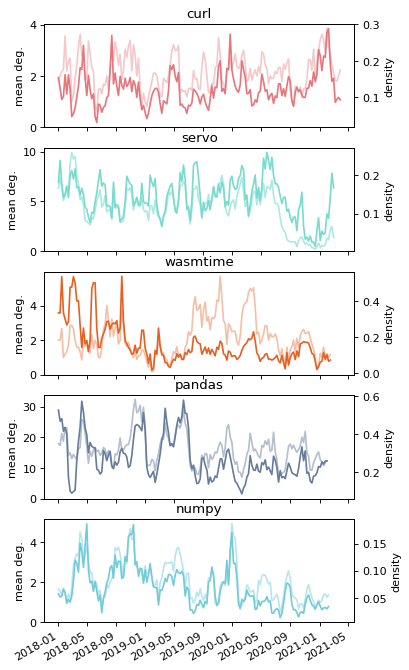
\includegraphics[width=\textwidth]{figures/qualitative/mean_deg_density/mean_deg.png}
        \caption{Density (dark) and mean degree (light).}
        \label{fig:density_a}
    \end{subfigure}
    \begin{subfigure}{0.46\textwidth}
        \centering
        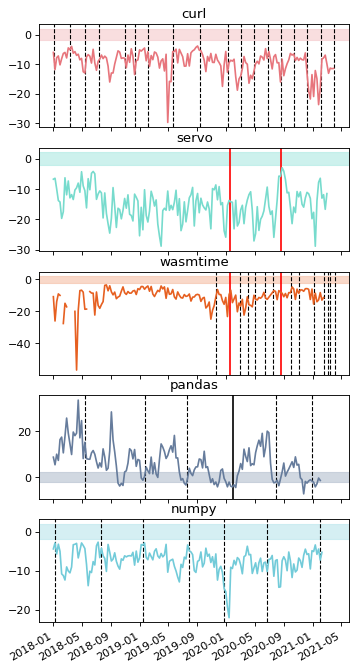
\includegraphics[width=\textwidth]{figures/qualitative/mean_deg_density/mean_deg_z_values.png}
        \caption{Z-values for density and releases.}
        \label{fig:density_b}
    \end{subfigure}
    \caption{Network density, mean degree and Z-values over time with significance threshold highlighted.}
    \label{fig:density}
\end{figure}

In order to adjust the network statistics for their sizes, we compare the network with a randomly generated, same-sized network. If we see a significant difference between the two values, we can confidently state that the changes we observe in the network statistics are independent of the network size. To measure the significance, we calculate the \textit{Z-value} of the actual network statistic and a 'general' network of the same size. In our implementation, we randomly generate ten networks with the same number of edges and nodes as the original network and use them to calculate the Z-value. The Z-value's formula is:

\[ Z=\frac{x-\mu}{\sigma} \]

where $x$ is the actual value we are comparing (in this case, the network density), $\mu$ is the average network density of the randomly generated networks, and $\sigma$ is the standard deviation of the random graphs. We consider a network significantly different from a random network if its Z-value is greater than $2$ in absolute terms. When the Z-value of network density is lower than $-2$, the network has a lower density than a same-sized general network, meaning the edges are more dispersed. Similarly, a Z-value greater than $2$ signals that the graph has more central hubs than the random network.

We plot the Z-values over time in Figure \ref{fig:density_b}, where the area between $-2$ and $2$ are colored to show at which times the network is significantly different from a randomly generated one: when the plotline is within this range, it is not significantly different; otherwise it is. In some cases, there is a break of continuity within the plot. This occurs when the standard deviation of the randomly generated network is $0$, which would result in a zero-division error. The standard deviation can only be $0$ when all the values are the same, which means our randomly generated networks have exactly the same density in these cases. This usually happens in extreme cases, when there is a very low number of nodes or edges.
  
Almost all projects have a significantly low network density, meaning that the edges are more distributed between the nodes. The notable exception is the \texttt{pandas} repository, which has an overall positive Z-value over time, with sometimes crossing the insignificant zone. These points are primarily troughs at the time of minor releases. We can also see on all projects that around a release, the Z-value approaches (or crosses) the threshold, which signals that the networks behave more like random networks around releases. The same can be observed for the layoff events, as \texttt{servo} gets close to $-2$ at the time of the announcement.

\subsubsection{Clustering coefficient}

The weighted global clustering coefficients explained in Section \ref{sec:clustering} is plotted over time in Figure \ref{fig:clust}. Because it would be difficult to show both the Z-values and the clustering coefficients on the same graph for each project, we only show the Z-values, as they both indicate the direction and the significance of the change. Where the clustering coefficient is significantly different from a random network to the negative side (meaning the Z-value at the corresponding date is less than $-2$) it drops below the highlighted $[-2, 2]$ area within each subgraph. Likewise, when there is a significant difference to the positive direction, the plot is above the highlighted area.

\begin{figure}[!htbp]
    \centering
    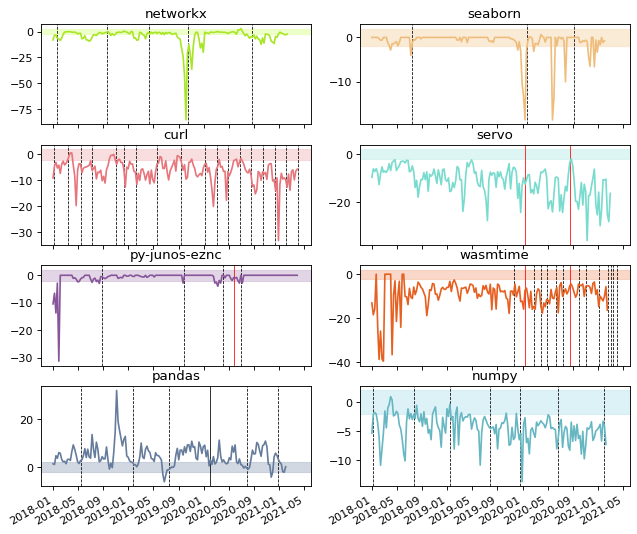
\includegraphics[width=\textwidth]{figures/qualitative/clustering_coeff/clustering_z.png}
    \caption{Clustering coefficient Z-values over time.}
    \label{fig:clust}
\end{figure}

We receive mixed results for the clustering coefficients. The smaller libraries (\texttt{NetworkX}, \texttt{seaborn} and \texttt{curl}) show a sudden spike before a release, which means that the network gets clustered before a release. However, the Z-value is always showing a negative sign being less than $-2$ in these cases (with the notable exception of \texttt{pandas}, which is mainly above $2$), signaling that the increase in clustering coefficient is significantly less than a same-sized random network. This shows that the spike and then a drop in the clustering coefficient before a release are caused by a sudden increase and decrease of activity within the project, but this activity is decentralized and affects all developers roughly the same. One of the reasons is the more decentralized workflow: as Crowston et al. \cite{crowstonHierarchyCentralizationFree2006} have identified, smaller projects early in their lifecycles tend to be more centralized, as there is less specialization to only one area of the project.

Interestingly, almost all the larger projects have lower clustering coefficients than a random network consistently, indicating a significant overlap of the edited files within the projects and less specialization. Another explanation could also be the use of shared files, which relates to the project structure. If an implementation of a new feature requires developers to edit almost all existing files by adding new functions, then the clustering coefficient will be low. On the other hand, if every new feature requires a new file to be added, developers will be mostly isolated in the collaboration network around the files, which will show up as a higher clustering coefficient than in a random network. This would explain why the \texttt{pandas} library has a positive Z-value consistently: the project structure does not require contributors to edit each other's files. Additionally, we can observe a drop in the clustering around releases but without statistical significance. This also confirms that the network becomes more random-like around releases. However, we can further extrapolate that a likely factor to this phenomenon is the feature integration: between releases, contributors center around their specialization editing only a limited number of isolated files, but before the release, the effort shifts towards integrating these features, which requires editing files outside the 'usual folder.'

\subsubsection{Mean path length}

Another measure that could be affected by a release is the length between nodes in the network. From an organizational perspective, a path between two contributors represents the information flow regarding a specific part of the project. If in a network every vertex tends to be close to the other nodes, meaning less jumps are required, they can gather information about a specific part of the project quicker. Smaller projects with fewer contributors naturally have relatively short connections to all other developers, and as the software gets larger with more contributors, the average shortest path between nodes is expected to get longer. However, if the project structure maintains central connecting 'hubs' (in this case: developers), the growth in length can remain lower.

In an undirected unweighted graph, the shortest path between two nodes is the least amount of edges needed to be touched to get from one node to the other. However, our collaboration network is a weighted undirected graph, where the edge weights represent the collaborative effort between two developers. A strong collaboration is represented as a higher edge weight, whereas a lower edge weight means there is less collaboration between the two contributors. The shortest path between two nodes in a weighted graph is the path with the least summed weight of the edges touched. In our case, we want to measure how far away each developer is from all the others to quantify the effort for reaching out to each other in case they want to involve a specific community member. To select the closest connection, we need to look for the strongest connection, meaning we have to consider the longest path between nodes.

\begin{figure}[!htbp]
    \centering
    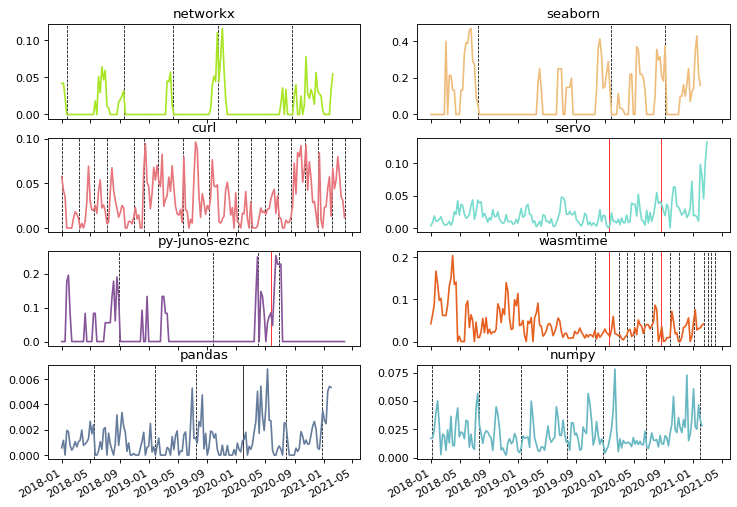
\includegraphics[width=\textwidth]{figures/qualitative/mean_path_length/path_length_all_normalized.png}
    \caption{Normalized mean longest path length over time.}
    \label{fig:mean_path}
\end{figure}

We calculate the average longest path $P$ by first summing up all the longest paths from a given node to all other nodes, then dividing by the number of connections, which is $n-1$ in a connected graph. Then we sum up all of these averages for all nodes, and divide by the number of nodes $n$:

\[ P = \frac{\sum{_{i=1}^{n}} \sum{_{j=1}^{n} -w_{ij}+1} }{n(n-1)} \]

where $w_{ij}$ is the edge weight between $a_i$ and $a_j$ in range $[0, 1]$. We multiply the weights by $-1$ and add $1$ in order to calculate for the longest, and not the shortest path. If there is no edge between $a_i$ and $a_j$, then $w_{ij}=0$.

To depict the changes over time in mean path length, we want to calculate the Z-value, just like with the other metrics. However, this proves to be difficult for the mean path length. When calculating the Z-value, we generate multiple graphs randomly, which have as many nodes and edges as the original, real network. Then we subtract the original value from the random graphs' average value and divide it with the standard deviation of the random network values. The issue rises with the standard deviation and division part: if all the randomly generated values happen to be exactly the same, their standard deviation will be $0$, which leads to a division by $0$ error. Different random values can only happen with the mean path if there are about the same edges as nodes in the network. In this case, random chains occur within the network, which are sometimes shorter, sometimes longer. Otherwise, either everyone is connected to everyone, and the mean path length is always $1$ when there are more edges than vertices, or nobody is connected to anyone, and there are never any changes in the reversed situation. Z-values cannot be calculated in either case, as all values at all points in time are the same.

This occurs for all eight projects when calculating the Z-value, and the graphs did not show any value. To circumvent this issue, we take an analytical approach to normalize our mean path length values. Instead of randomly generating the networks, we take the absolute possible largest mean path length in any network and divide each value with it. The maximum path length in any given graph is $(N-1)/2$, where $N$ is the number of developers in the network. We normalize the mean path length by dividing with this value, and the results are depicted in Figure \ref{fig:mean_path}.

It is visible in the smaller projects (\texttt{NetworkX}, \texttt{py-junos-eznc}, \texttt{seaborn}) that the path length increases before a release due to the increased activity, and otherwise it stays $0$. This indicates a 'push-type' release process, where the releases are sporadic, and a new release is created to incorporate and deploy the changes implemented. With the other projects, we do not see any correlation between releases and mean path length.

\subsubsection{Core and periphery analysis}

Around releases, it is reasonably expected that the ratio between core and periphery developers changes. It has already been established that within a project, the core members tend to stay the same throughout the project's lifecycle, but the tasks regarding the new release preparation might change their relationship with the periphery community members. The first method we use to identify core members is explained in Section \ref{sec:deg_centrality}. We call the number of core members identified this way as \textit{Degree centrality core} value. 

Besides taking the 20th percentile of the leading clustering coefficients to identify the number of core developers in the network, we also use the degree number of each developer to identify their \textit{K-core value}. The K-core of a network is the subset of nodes, which have at least $k$ degrees, and we call the network's K-core value the number of nodes within the K-core \cite{batageljAlgorithmCoresDecomposition2003}. Then, we identify the vertices, which are in the top 20th percentile of K-cores, as core developers. For example, if the maximum number of degrees within the network is 10, then the K-core value is the number of nodes with at least a degree number of 8.

We observe the ratio between the number of core and periphery developers by dividing the number of core developers by the number of nodes within the network. This gives us a ratio between $0$ and $1$ for both the \textit{Degree centrality core} and the \textit{K-core value} methods, where $1$ means the network only contains core developers. It is important to note that the only case both methods can have $0$ as a core/periphery ratio is when there is no collaboration within the network and all nodes are isolated with a degree of $0$. We then plot the Z-values for both methods' core/developer ratio as before, which can be seen in Figure \ref{fig:core-periphery}.

\begin{figure}[!htbp]
    \centering
    \begin{subfigure}{0.99\textwidth}
        \centering
        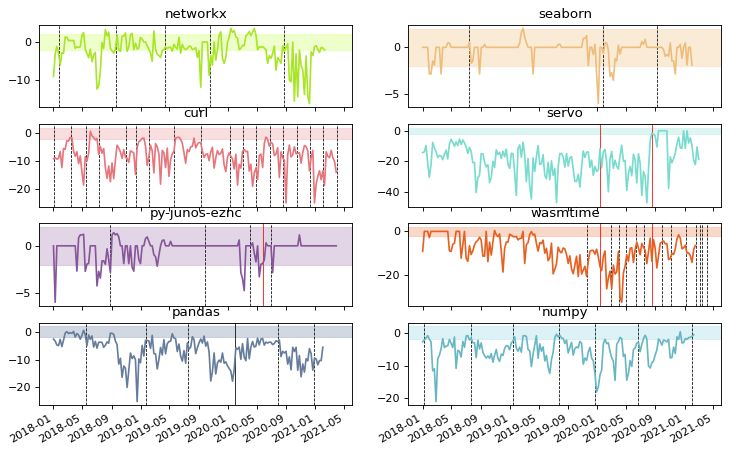
\includegraphics[width=0.99\textwidth]{figures/qualitative/core_periphery/core_periphery_k_core.png}
        \caption{Core/periphery K-core method}
        \label{fig:cp-k-core}
    \end{subfigure}
    \begin{subfigure}{0.99\textwidth}
        \centering
        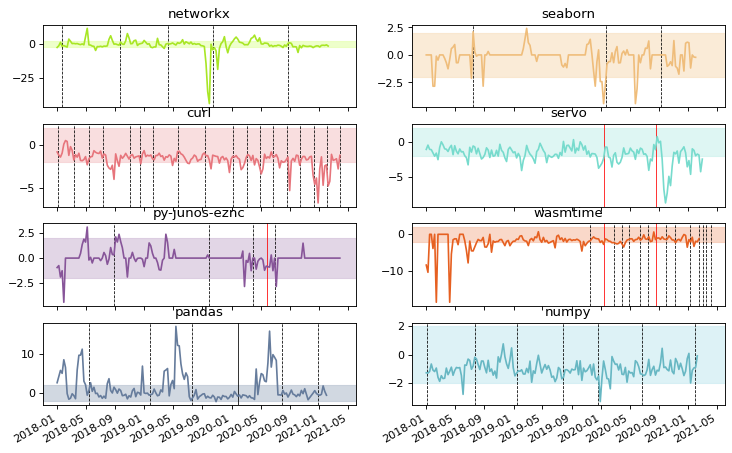
\includegraphics[width=0.99\textwidth]{figures/qualitative/core_periphery/core_periphery_degree.png}
        \caption{Core/periphery degree centrality method}
        \label{fig:cp-degree-centrality}
    \end{subfigure}
    \caption{Core/periphery ratio's Z-value over time with K-core and Degree centrality methods.}
    \label{fig:core-periphery}

\end{figure}

Figure \ref{fig:cp-k-core} depicts the core/periphery ratio calculated with the K-core method, and Figure \ref{fig:cp-degree-centrality} shows the degree centrality method. We can see a sharp difference between the smaller and larger projects again. For the smaller projects, the two measures roughly behave the same, as their plots overlap most of the time. Most of the time, these values stay within the statistically insignificant range and only in these cases are significantly different from a random network.

In contrast, the large projects have their K-core ratios consistently below $-2$, indicating that the core ratio is consistently lower than a randomly generated network, which signals its centralized property. This cannot be said for the Degree centrality core ratios, which are consistently within the insignificant range. Just as with the smaller projects like \texttt{NetworkX}, \texttt{seaborn} and \texttt{py-junos-eznc}, we can observe a significant drop in K-core ratio Z-values within 2 to 3 months after the release. The difference between the two networks is demonstrated for \texttt{NumPy}'s minor release on 22.12.2019, where the networks for 1-month after and 1-month before are contrasted in Figure \ref{fig:core-periphery-numpy}.

\begin{figure}[!htbp]
    \centering
    \begin{subfigure}{0.49\textwidth}
        \centering
        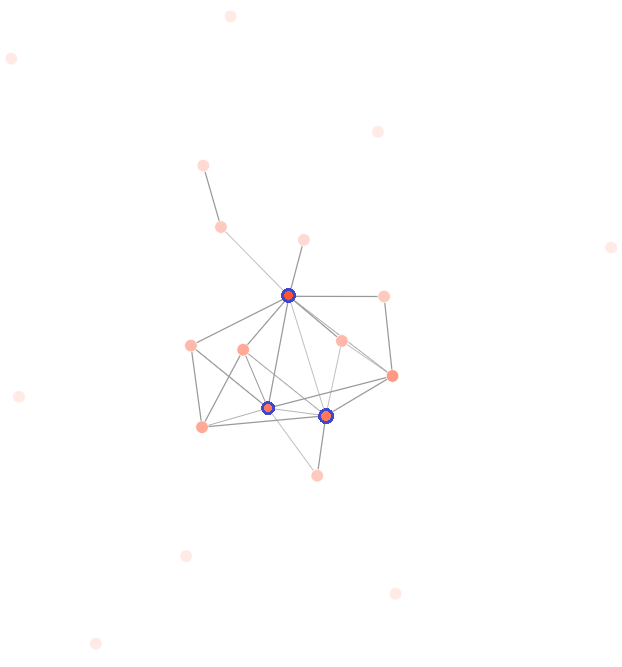
\includegraphics[width=\textwidth]{figures/qualitative/core_periphery/numpy_before.png}
        \caption{Between 2019-12-09 and 2020-01-06}
        \label{fig:numpy-before}
    \end{subfigure}
    \hfill
    \begin{subfigure}{0.49\textwidth}
        \centering
        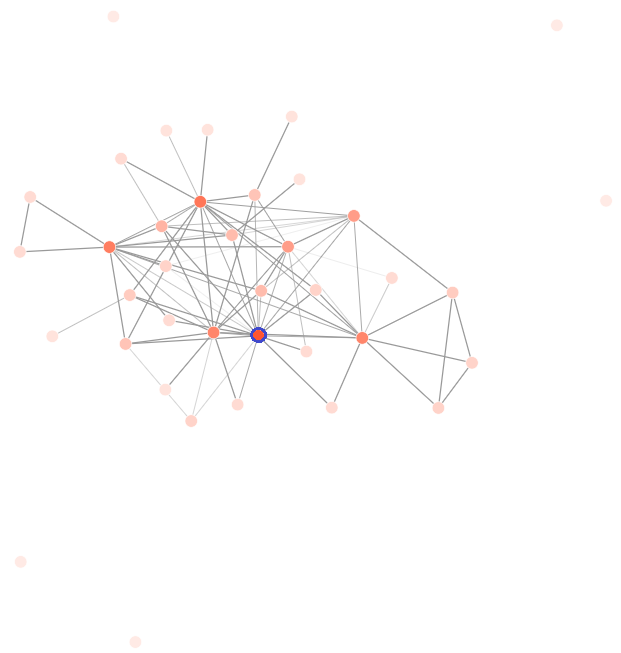
\includegraphics[width=\textwidth]{figures/qualitative/core_periphery/numpy_after.png}
        \caption{Between 2020-01-06 and 2020-02-03}
        \label{fig:numpy-after}
    \end{subfigure}
    \caption{\texttt{NumPy} collaboration network before and after the 2020-12-22 minor release, depicting how the network becomes more numerous, it is also becoming more centralized.}
    \label{fig:core-periphery-numpy}
\end{figure}

The nodes identified as core are highlighted in blue. In Figure \ref{fig:numpy-before}, we can see that the maximum number of degree is paired with a couple of similarly connected nodes, and this is combined with a relatively small number of nodes in the graph, which results in a relatively high number of core members with a low number of periphery developers. Therefore, the ratio gets higher, which is more similar to an almost completely dispersed random network. Whereas in Figure \ref{fig:numpy-after}, we can observe the opposite: the small number of core members (only one) is combined with numerous nodes, which creates a low core-periphery ratio that is significantly lower than in a randomly generated same-sized network. The fact that the second graph has more nodes than the first, and they are more connected lets us conclude that the increase in activity is the effect of the release, where after the new version release to the public led to an increase in bug reports, which caused a surge in activity as they are being fixed.

The notable exception for the K-core values in Figure \ref{fig:core-periphery} is again \texttt{pandas}, where the Degree centrality core-periphery ratio determines each release nicely: we can consistently see a positive spike above the significance level 2 months before each release. This finding is consistent with the degree centrality analysis; however, here, it is more pronounced. The drop after the release in the K-core ratio also seems to hold true.

In general, we can say that, especially in larger projects, the core can be separated from the periphery developers, as the Z-values show significantly lower values than of a random network regarding the core/periphery ratio. We can also observe in projects with more contributors that a release causes the Z-values to rise, which indicates that the graph becomes more even. We can conclude from this observation that more periphery contributors are active around a release, confirming the theory that an upcoming release triggers more activity as developers want to push their changes to the upcoming release.

\subsubsection{Hierarchy}

As the last step, we take a look at the hierarchy of the networks over time. We use the method described in Section \ref{sec:hierarchy}, and we plot the linear regression's $\beta_1$ value (the slope of the trendline). Figure \ref{fig:hierarchy_all} shows these values over time per observed project, where the highlighted area indicates the zone where the Z-value is not significant.

\begin{figure}[!htbp]
    \centering
    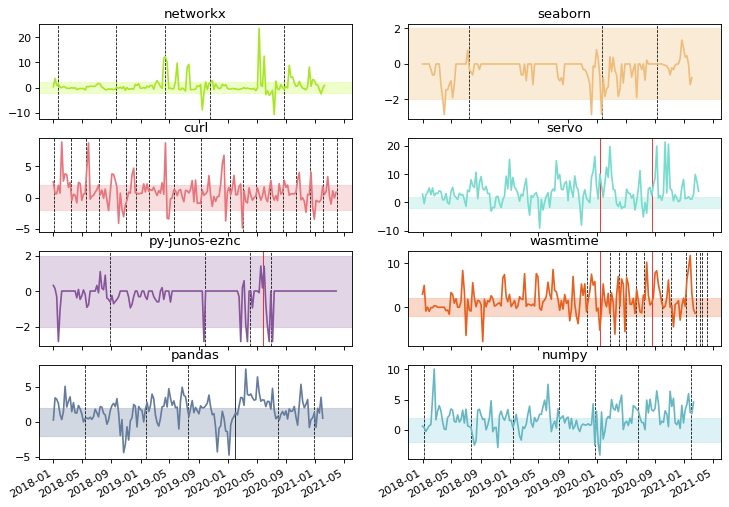
\includegraphics[width=\textwidth]{figures/qualitative/hierarchy/hierarchy_all_z.png}
    \caption{Hierarchy over time}
    \label{fig:hierarchy_all}
\end{figure}

In \texttt{NetworkX} and \texttt{seaborn} we can see activity only around releases, which is due to the fact that there are not enough commits and developer activity to form a collaboration network properly, so it defaults to zero. Therefore, we can contribute the hierarchy change in their cases to the change in network size.

Just as with the other statistics, \texttt{curl} has a frequent and regular release plan, which makes it hard to observe any regularities around releases. We can see some spikes and some troughs coincidentally at the same time as the releases, but there is not any consistency between them, and therefore we cannot conclude a definitive cause and effect between hierarchy and releases. Unlike the other projects, \texttt{curl} has a lower hierarchy score as it drops below $0$ many times, indicating a somewhat more hierarchical structure. This is expected, as it is known that it is mainly developed by a single developer, which results in a high hierarchy.

In case of \texttt{servo}, \texttt{py-junos-eznc} and \texttt{Wasmtime} the hierarchy seems to correlate with the unexpected events closely. In \texttt{servo} there is a definitive spike exactly at both after the first layoff event and exactly at the second layoff event, which indicates a huge change in the network. Similarly, \texttt{py-junos-eznc} also shows the only significant Z-value at the time of the layoff event with a positive spike. \texttt{Wasmtime} also shows a positive spike at the exact time of the layoff, which leads us to conclude that the sudden decline of hierarchy (it is more hierarchical if the value is negative) is a good indicator of the layoff events. This can be explained by removing core contributors, as the teams are disrupted, and developers have to collaborate directly with more of their peers, as opposed to going through the established channels.

\subsection{Release regularity}
\label{sec:release_reg}

During the network measure analysis, we recognized that the regularity of the releases could significantly affect how it changes the network. For example, a push model can be recognized in smaller projects, where the new features are added, and then a new release is created, which incorporates this feature. This ensures that the new feature gets deployed as fast as possible. In these cases, we can see that the releases do not happen regularly, but there is a significant change before or after it when there is a release.

Projects that follow a pull model tend to have more regular release periods, and they are also the large projects in our analysis. Within these projects, the flow of new features and bug fixes are constant, and they are deployed within a fixed period of time. Therefore, the new release does not necessarily have a visible impact on the network because if the feature is not complete yet, it will be released in the next one. An excellent example for this is the \textit{1.0} release of \texttt{pandas}, which does not show any more network change in any metrics compared to a minor release despite being the only major release within all eight projects — contrary to the expectations.

In order to quantify the regularity of the releases within the project, we calculate the \textit{coefficient of variation} (CV) within each project for the days between each release. The $CV_i$ is the ratio of the standard deviation $\sigma$ to the mean $\mu$ of the number of days passed between two releases for project $i$, which can also be interpreted as a percentage \cite{everittCambridgeDictionaryStatistics1998a}:

\[ CV_i = \frac{\sigma_i}{\mu_i} \]

It must be determined for each type of release because we have seen that the type can affect regularity. For example, in some projects, patches follow up on a minor or major release, making the overall releases irregular, even though major and minor releases could still follow a regular pattern. We measure the release regularity CV in Table \ref{tab:regularity}. In order to calculate the value, the project must have at least two releases per type to have at least one value for days passed between releases. In cases when this condition is not met, we leave the values empty.

\begin{table}[!htbp]
    \centering
    \resizebox{\textwidth}{!}{%
        \begin{tabular}{| l | c | c | c | c | c | c | c | c |}
            \hline
            \multirow{2}{7.5em}{\textbf{Project name}} & \multicolumn{4}{|c|}{\textbf{Minor+Major releases}} & \multicolumn{4}{|c|}{\textbf{Patch releases}} \\
            \cline{2-9}
            & \textbf{$N$} & \textbf{$\sigma$} & \textbf{$\mu$} & \textbf{$CV$} & \textbf{$N$} & \textbf{$\sigma$} & \textbf{$\mu$} & \textbf{$CV$} \\
            \hline
            \texttt{pandas} & 6 & 34.93 & 191.2 &\textbf{0.1827} & 21 & 47.72 & 48.15 & \textbf{0.9911} \\
            \texttt{NumPy} & 7 & 22.91 & 186.67 & \textbf{0.1227} & 29 & 22.44 & 40.39 & \textbf{0.5554} \\
            \texttt{NetworkX} & 5 & 46.70 & 235.75 & \textbf{0.1981} & 1 & - & - & \textbf{-} \\
            \texttt{seaborn} & 3 & 164.5 & 392.5 & \textbf{0.4191} & 3 & 71.5 & 166.5 & \textbf{0.4294} \\
            \texttt{curl} & 18 & 24.19 & 69.53 & \textbf{0.3479} & 8 & 99.29 & 136.0 & \textbf{0.7301} \\
            \texttt{servo} & 116 & 8.31 & 8.67 & \textbf{0.9585} & 189 & 4.99 & 5.05 & \textbf{0.9876} \\
            \texttt{Wasmtime} & 13 & 24.49 & 41.91 & \textbf{0.5843} & 1 & - & - & \textbf{-} \\
            \texttt{py-junos-eznc} & 4 & 127.68 & 224.33 & \textbf{0.5692} & 10 & 84.51 & 117.44 & \textbf{0.7196} \\
            \hline
        \end{tabular}
    }
    \caption{Release regularities for major, minor and patch releases.}
    \label{tab:regularity}
\end{table}

The coefficient of variation has a lower bound of $0$ in our case because the number of days passed between two releases can never be a negative number — the smallest possible is $0$ when the release dates are exactly the same days apart from each other. However, the CV has no upper bound, as the standard deviation can be arbitrarily large and larger than the mean release days. Also, there is no unit associated with it, so we can only give meaning to the CV value in the context of other projects as a comparison: a project with a smaller CV value has a more regular deployment schedule than another one with a higher CV. Since its scale is a ratio scale, we can also interpret a two times larger value as two times more regular interval.

We also note that although the coefficient compensates for the difference between mean values, it does not take into consideration the number of intervals observed. This means that a one-day delay of a release from an established schedule does not have an enormous impact when there are 100 other releases on time, but if there are only four releases, this changes the mean significantly and, therefore, the CV too. This is why we also display the number of releases as $N$. \\

It can be observed in all projects that the minor and major releases are more regular than the patch releases. This confirms the theory that patch releases are mainly added as bug fixes for minor and major releases after they are made public, and they do not follow a regular pattern. The difference between patches and major-minors are not consistent within the repositories: the greatest difference is in \texttt{pandas}, where the patch CV is five times larger than the minor-major CV. Close second is \texttt{NumPy} with a similar 4.6 times larger irregularity of patches. Both projects have roughly a 180-day release cycle, and it is clearly visible that patches directly follow the minor releases in Figure \ref{fig:nnodes}, and they get sparser as we get further away from the minor releases in time.

The repositories \texttt{NetworkX} and \texttt{Wasmtime} do not have enough patches within the observed period to calculate the patch values, therefore we cannot compare them to the major-minor releases. The \texttt{NetworkX} repo has a much more regular minor release cycle than \texttt{py-juno-eznc}, which has a similarly large release cycle of about 230 days. This indicates that small-sized projects, which usually have longer release cycles, can also vary a lot depending on the project, and they can be just as regular as a larger repository. \texttt{Seaborn} is somewhere in between the previous two in terms of regularity, however, with only 3 minor and 3 patch releases, we cannot say any definite about comparing it to other projects, because we cannot say for sure that the middle release of the 3 is an outlier of the many regular releases, or it is completely random even if we go back further in time to check a larger number of releases.

\texttt{Curl} has one of the shortest minor release cycles with an average of 70 days, and it is regular with a CV of $0.35$, which confirms what we have observed visually in Figure \ref{fig:nnodes}. A short but regular release cycle will result in more added releases over a fixed time period, which leaves room for more errors. Furthermore, with a short release cycle only a small delay is required to have a great impact on the CV value. Therefore, we believe that this method could be biased towards small release cycles, and they are shown as less regular than a larger, 180-day cycle shows. Nevertheless, it is still clear from the coefficient that \texttt{curl} is one of the regular projects.

\texttt{Servo} has an extremely short release plan with only an average of 8-9 days between minor releases. We can also see the bias against shorter cycles, as it has by far the largest coefficient of variation with $0.96$. Due to the short time between releases, it is enough to delay a release by just a couple of days to significantly worsen the CV score. However, with a standard deviation also being around 8, we can see that the regularity cannot be as precise as in \texttt{pandas} or \texttt{NumPy}, despite the bias. \\

Considering the plotted graphs with the releases and also the CV values, we want to determine a CV value that can classify a project into 'regular' or 'irregular' release cycles. We have seen a slight bias against shorter cycles, but finding a way to compensate for it would greatly increase complexity, which could lead to other issues. Therefore, we will use a coefficient of variation of $0.4$ \textbf{for the minor and major releases} to draw the line: every value below that indicates a regular release plan, and everything above that signals an irregular cycle. As stated before, patches tend to follow up on majors and minors; therefore, we should not consider them overall.  By this classification, \texttt{pandas}, \texttt{NumPy}, \texttt{NetworkX} and \texttt{curl} are \textit{regular}, whereas \texttt{seaborn}, \texttt{servo}, \texttt{Wasmtime} and \texttt{py-junos-eznc} are \textit{irregular} when it comes to release cycles. We can also see visually on the plotted graphs in Section \ref{sec:releases} that this separation seems to be right.

\subsection{Release efficiency, issues}

So far, we have seen how the collaboration network statistics change before, at, and after a release. We also categorized the releases based on major, minor, and patch releases, where we expected more significant changes in collaboration with a larger release — which was not always the case. Then we categorized the projects into regular and irregular release cycles. As a next step, we want to analyze whether a release is successful or unsuccessful and how we can measure this success rate.

The common perception of software development is that a rushed release will have worse quality, which will result in more bugs in the software. This was confirmed by Michlmayr et al. \cite{michlmayrWhyHowShould2015}, and they name the lack of testing as one of the primary sources of rushed code. They also identify the two release strategies we mentioned in Section \ref{sec:release_reg}, namely regular, time-based, or irregular, feature-based release strategies. They have found that a feature-based strategy can cause rushed code development and poorly tested features due to the fact that the next release date is unknown. Therefore, contributors are incentivized to submit their changes as soon as possible so that their changes are deployed to the public users of the open-source software. This unpredictability forces developers to skip or glance over the testing phases, leading to more bugs in the software.

A fixed time-based release cycle, on the other hand, is predictable, which allows contributors to plan ahead the tasks related to the new feature or bug fixes \cite{michlmayrWhyHowShould2015}. Furthermore, in case of a delay, it can be already known when the next one will be approximately, and additional features can be replanned accordingly. Therefore, a regular release schedule is a sign of a healthy project, which indicates to the users that there is active support for the OSS software and developers that the project is set for a longer-term, and it is a viable candidate to contribute into.

As a new version is released, the users of the software are notified through the distribution channels, which triggers a spike in downloads due to users wanting to be up-to-date to the latest software version \cite{khomhFasterReleasesImprove2012}. Due to the quick adoption period within FLOSS projects, most bugs are also expected to be reported shortly after a release, with a rushed version possibly having a larger amount of bugs after its release. Therefore, a great measure of release quality can be the number of bugs reported after a release. GitHub's standard bug and feature tracking API is the Issues page, so the number of issues created will be used for this purpose. 

\subsubsection{Issue opening and closing frequencies}

The number of issues opened and closed can be seen in Figure \ref{fig:issues_created_closed}. The issues are sampled every 14 days, where the seven days before and after are aggregated, separately for issues closed and issues created. For example, the month of January will have two data points: January 8, which aggregates the period January 1-14, and January 22, which will sum up all the number of issues created and closed between January 15-28.

\begin{figure}[!htbp]
    \centering
    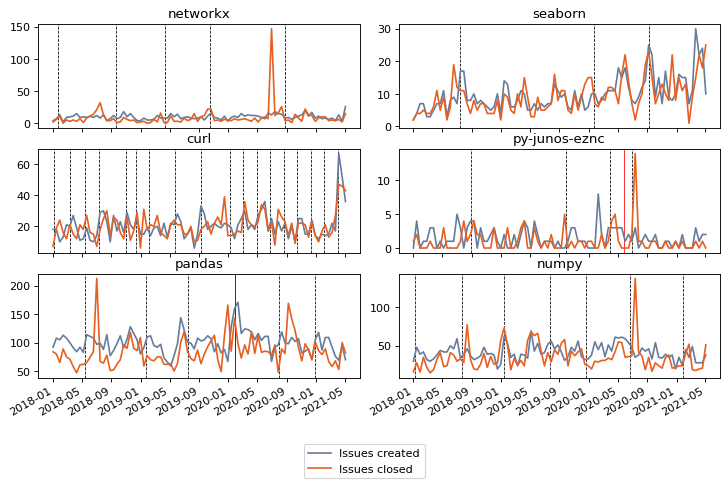
\includegraphics[width=\textwidth]{figures/qualitative/issues_closed_created/issues.png}
    \caption{Issues closed and created per project.}
    \label{fig:issues_created_closed}
\end{figure}

Based on the plots, we can confirm the increased number of issues at a release, as all projects' most release dates coincide with a peak in issues created. Interestingly, the peaks do not necessarily come after or exactly at the release, and sometimes they precede the actual release date. Some examples are the \texttt{pandas} version \texttt{v0.24.0} on \textit{January 25, 2019}, or version \texttt{v0.25.0} on \textit{July 18, 2019}, or \texttt{py-junos-eznc}'s \texttt{2.3.2} on \textit{April 1, 2020}. Most likely, this is an effect of successful testing: before the release, the software is thoroughly tested, and all identified bugs are registered as issues. Since most issues are fixed before the release, users do not find more issues than usual; therefore, the issues created drop. Similarly, a peak in opened issues after the release might mean a less robust testing system. We can observe this in \texttt{NetworkX}, where the number of issues created gets higher at the release or shortly after.

The number of issues closed follows a similar trend. The expectation was that the issues closed peak before a release, since the planned tasks to be added to the new version are being closed, and after the new release, the issues closed would fall, as most features and bugs have already been implemented in the new version. Although this holds true in some cases, especially in \texttt{NetworkX} and \texttt{pandas}, this is not the case all the time, as sometimes large spikes occur right after a release, such as \texttt{NumPy}'s version \texttt{v1.19.0} on \textit{Jun 20, 2020}, or \texttt{pandas}' new release on \textit{May 15, 2018}. We assume that unusually large spikes like these occur as a 'clean-up' after the release to plan the new release cycle.

\subsubsection{Open issues over time}

Now that we have seen some regularities regarding issue creation and close, we also examine how the number of open issues changes with the releases. However, as we discussed in Section \ref{sec:project_issues}, since there are continuously open issues in an active project, some of which are not closed at the time of taking the project snapshots, we cannot take any averages or aggregation due to the survival bias.

Figure \ref{fig:open_issues} shows the number of open issues for each project in the observed three years. We can see that in almost all projects, the number of open issues steadily rises, with smaller dips occurring around some but not all releases. This shows that maintaining and organizing the issues becomes a more considerable challenge as the project grows and confirms the large spikes in the number of issues closed in Figure \ref{fig:issues_created_closed} that these are 'clean-up' events, where the backlog is decluttered by closing the obsolete issues.

\begin{figure}[!htbp]
    \centering
    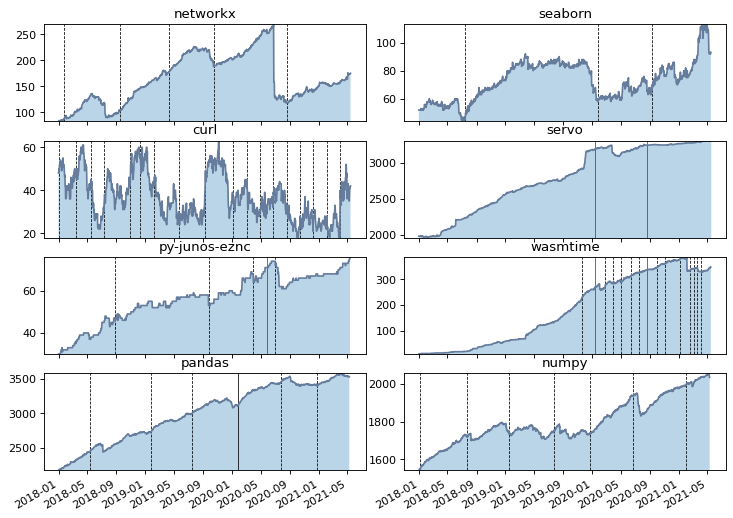
\includegraphics[width=\textwidth]{figures/qualitative/issues_closed_created/open_issues.png}
    \caption{The open issues keeps steadily increasing in almost all projects.}
    \label{fig:open_issues}
\end{figure}

The only exception from the ever-growing number of open issues is the \texttt{curl} library, which manages to keep the number of open issues below 60, despite being the oldest project of all eight subject to our analysis. This could also be related to the short release cycle. As Khomh et al. \cite{khomhFasterReleasesImprove2012} have found, bugs are fixed significantly faster with rapid release plans. Furthermore, as \texttt{curl} is the most centralized project, with one single main developer, issue management is much more efficient, as there is no need for group discussions and prioritization between developers. Interestingly, \texttt{servo} has the shortest release timing strategy, with sometimes multiple minor releases in a week. Yet, it is still struggling with the increasing number of issues, indicating that a strongly centralized organizational structure can have a much heavier weight in the increase of open issues over time.

\subsubsection{Bugs and features}
\label{sec:bugs-features}
Issues can describe many tasks within a project, such as ideas, features, discussions, bugs, warnings, and depreciation plans. Each repository organizes the issues with labels, which can be created and color-coded freely within each project. Therefore, the labels cannot be used across projects, as each repository has its own personalized system. For example, \texttt{pandas} uses the tag 'Bug' for bugs, \texttt{NumPy} uses '00 — Bug', since they order the labels by giving a number in front of it, and \texttt{servo} does not have a bug category because they divided this category into 'I-crash' and 'I-wrong' among other labels. Also, they categorize the labels by their starting letter, which is not a practice in the other projects.

Seeing which types of issues are affected the most by a release could also provide insight into how the project, and by extension, the collaboration network changes. Instead of using the labels, we categorize them with pattern matching in the title as described in Section \ref{sec:project_issues} with the same keywords and method. Even though the matching rate is not expected to be high, we can still apply the method for the projects because the issues matching a category have a high chance of actually belonging to that category due to the low number of keywords being used, meaning our false-positive rate for the classification is presumably low. However, we cannot confirm this, as the manual effort to classify the issues would be too large. The results can be seen in Figure \ref{fig:open_bugs_features}.

\begin{figure}[!htbp]
    \centering
    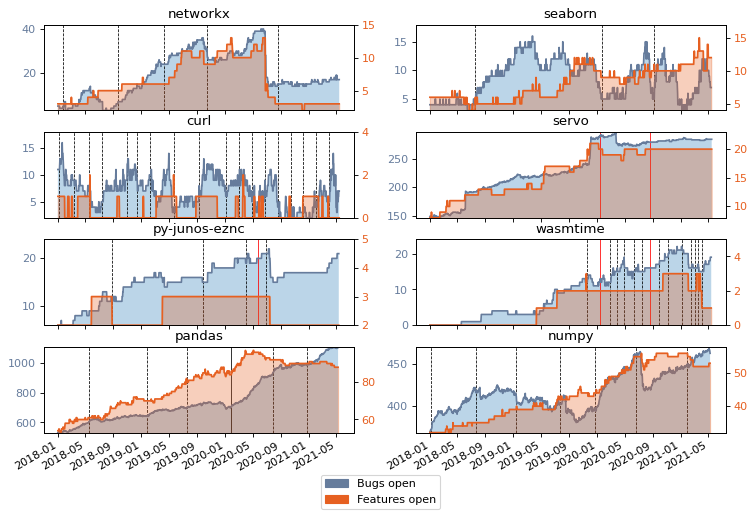
\includegraphics[width=\textwidth]{figures/qualitative/issues_closed_created/features_and_bugs.png}
    \caption{The number of open bugs and features mostly overlap, with some exceptions.}
    \label{fig:open_bugs_features}
\end{figure}

The bugs and features are presented on two different scales because their magnitude is different (there are much more bugs identified than features), but we want to compare the relative changes to each other. Sadly we cannot see any significant difference between the number of bugs and features open, apart from a few exceptions, such as the December 2020 release of \texttt{pandas}, after which the number of open features declines while the number of bugs rises; or the July 2019 version of \texttt{NumPy}, where the opposite is true and the features keep rising while the bugs decline.

Since both the features and the bugs curves follow the same shape, which is also the same as the overall shape of the issues, we cannot draw any definitive conclusions regarding the difference between bug and feature issues. The reason for this is that we are only able to classify a small portion of the issues. When the overall number of issues rises, it makes it more likely to find a feature or bug just by sheer luck, and that is why both curves follow the overall curve. Therefore, we cannot confirm the statement that there is no difference either.

\begin{table}[!htbp]
    \centering
    \resizebox{\textwidth}{!} & N & \textit{\%} & N & \textit{\%} \\
            \hline
            \texttt{pandas} & 20501 & 6245 & \textit{30.46\%} & 294 & \textit{1.43\%} & 13962 & \textit{68.10\%} \\
            \texttt{NumPy} & 9536 & 2421 & \textit{25.39\%} & 134 & \textit{1.41\%} & 6981 & \textit{73.21\%} \\
            \texttt{NetworkX} & 2524 & 384 & \textit{15.21\%} & 54 & \textit{2.14\%} & 2086 & \textit{82.65\%} \\
            \texttt{seaborn} & 1885 & 341 & \textit{18.09\%} & 99 & \textit{5.25\%} & 1445 & \textit{76.66\%} \\
            \texttt{curl} & 2866 & 489 & \textit{17.06\%} & 35 & \textit{1.22\%} & 2342 & \textit{81.72\%} \\
            \texttt{servo} & 11485 & 1016 & \textit{8.85\%} & 57 & \textit{0.50\%} & 10412 & \textit{90.66\%} \\
            \texttt{Wasmtime} & 917 & 72 & \textit{7.85\%} & 6 & \textit{0.65\%} & 839 & \textit{91.49\%} \\
            \texttt{py-junos-eznc} & 475 & 106 & \textit{22.32\%} & 5 & \textit{1.05\%} & 364 & \textit{76.63\%} \\
            \hline
            \textbf{Overall} & \textbf{50189} & \textbf{11074} & \textit{\textbf{22.06\%}} & \textbf{684} & \textit{\textbf{1.36\%}} & \textbf{38431} & \textit{\textbf{76.57\%}} \\
            \hline
        \end{tabular}
    }
    \caption{Issue classification results. The vast majority of issues could not be classified with the proposed keyword-based classification.}
    \label{tab:issues_class}
\end{table}

We summarize the classification results in Table \ref{tab:issues_class}. The vast majority of issues could not be classified, and on average only 23\% can be identified as either bug or feature. Especially the feature recognition has the worst performance with a mere 1.36\% of all issues on average. Although we believe that bugs should be more numerous within all repositories compared to features, our expectation is higher than the results we are seeing. We suggest for future research applying text mining techniques on not just the issue title but also on the description. Additionally, duplicates could be filtered, and sentiment analysis could be conducted on the issue title, description, and received comments. However, these tasks are out of scope for the extent of our analysis.

\subsection{Results}

In our qualitative analysis, we identified the primary metrics of a collaboration network and observed these metrics in 8 hand-picked projects. Choosing a wide range of repositories in size, centralization, and release plans was a crucial criterion. We gathered each project's release over three years and classified them as major, minor, or patch releases based on their semantic versioning. Furthermore, we added the 'unexpected' events to this list for some selected repositories, as we also wanted to observe the layoff events and their effects on the network.

We looked at the number of commits, and we could identify that a project is active by the relative number of commits in a time period. For example, \texttt{servo} has a significantly reduced number of commits after the second, more significant layoff wave. We also observed the number of nodes within the network rise in specific projects before a release, indicating an uptick in activity. In order to normalize the network size and compare each project to each other, we introduced the Z-value, which tells us whether the measured value is significantly higher or lower than in a random network with the same number of edges and nodes.

The Z-values are consistently lower in almost all projects for network density, mean degree, clustering coefficient and mean path lengths, but the \texttt{pandas} library is an exception, as it tends to be positively different from a random network. This signals a stronger centralization and more organizational effort than in other repositories. Although \texttt{curl} is also very centralized as it is known that the primary support comes from one developer, since everyone is centered around the main developer, it is not significantly different from other projects, where it is centered around a core developer network, thus implying \texttt{pandas} having multiple cores, which produce multiple central clusters within the network.

The number of overall contributors in a repository, which is a proxy for their size, also greatly affects the collaboration network. In smaller projects, activity tends to happen before a release, but in between releases or events, even the 28-day time window proves to be too small to create a network that consists of more than just one or two developers working in isolation. Therefore, the network metrics are flat in these projects, and they only show activity before a release. In large projects, where there is a constant level of activity, the measures are inconclusive, as there are not any single metric whose change consistently coincides with a major or minor release for all projects. Clustering coefficient and network density seem to work well in the case of \texttt{pandas}, and the network density and the core/periphery ratio are also good predictors in \texttt{NumPy}, but not for the rest.

Regarding the layoff events, hierarchy proved to be the best predictor, as all events coincided with a spike in hierarchy towards more decentralization. This is justified by removing the core members, as it naturally creates a more decentralized network. Also, hierarchy is a good predictor of releases in some cases, for example, for some \texttt{pandas} releases, but not as significant as for the layoff events.

We have also seen that the repositories have varying release scheduling and strategies. Therefore, two parameters were identified: whether they follow a regular or irregular release schedule and if there is a regular schedule, what is the time difference between two versions. We measured the regularity with the elapsed time periods' coefficient of variations and identified the threshold of $0.4$, below which a repository is considered as having a regular schedule, and above it is irregular.

Having a short release plan can obscure the changes in the network statistics, which could be one of the reasons why we cannot identify any metrics that predict well the new versions of \texttt{curl} and \texttt{Wasmtime} libraries. Furthermore, according to the state-of-the-art literature, a regular deployment cycle makes the release planning more predictable, therefore, causes more minor changes in the collaboration metrics. We have found that all large and medium projects (\texttt{servo, curl, Wasmtime, pandas, NumPy}) have adopted a regular release plan, while the small repositories have not. This leads to the conclusion that switching to a regular release plan is a natural step in an OSS's lifecycle, and it is a sign of a healthy and mature project. \\

To discover the relationship between releases and issues, we observed the number of issues opened and closed with each new version. We expected that significantly more issues are closed before a release due to the bug fixes and features being included in the next version, and significantly more are opened after it because of the newly discovered bugs and feature ideas after a release is made public. We found this to be true for irregular release schedules, where the availability of a new feature prompts a new version and not due to reaching a new release time. In repositories that have adopted a regular release strategy and tend to be more mature, however, the opposite can be observed. Due to rigorous testing before a release date, issues are created before a new version is available, and they are closed within a clean-up process after the release is made publicly available.

Issue clean-ups usually happen around releases, but this is not necessarily the case in every project. When analyzing the number of open tickets, we noticed that the number of open tickets grows over time in almost all projects. As an effort to keep the number of open issues manageable, sometimes project organizers close a significant amount of tickets at once, causing a spike in the number of closed issues. However, only \texttt{curl} seems to be able to keep the open issues at a constant level, which we contribute to having only a single developer as a core member, which eliminates the necessity to discuss, prioritize and triage open issues.

In order to confirm the theory that the number of bugs increases after a release, we classified the issues into bugs and features based on keywords and pattern-matching. However, due to the heterogeneous nature of issue categorization and labeling, we could only classify a small percentage of issues. This caused the number of bugs and features to be tied to the overall number of issues: when the number of open issues increases, we are more likely to find and classify a bug and a feature, so their numbers will also rise. This effect ties the number of both bugs and features to the overall number of issues, so their shapes look approximately the same over time, and we are not able to draw any conclusions from them. As further analysis is out of scope for our work, we suggest a more robust classification method for bugs and features with text mining tools, such as natural language processing (NLP), for not just the titles but also the description and comments of the issues. Furthermore, sentiment analysis on the comment responses could provide more insight into how issues are resolved.

% CONCLUSION: qualitative research needed to observe correlations.

\section{Quantitative OSS project analysis}
\label{sec:quantitative}

In Section \ref{sec:patterns} we have seen how the heterogeneity of open-source projects makes it hard to draw conclusions from the network statistics over time. We have seen some correlations between the releases and the metrics, but they did not apply to all repositories. Furthermore, the relatively small number of repositories also prevented generalizing the findings, for example, the metrics, which proved to be effective in \texttt{pandas} like clustering coefficient or degree centrality, might also apply to the majority of open-source repositories, but our project choices did not include any that falls into this group. Therefore, in this section, we will conduct quantitative research on a large number of randomly selected repositories to rule out any bias we might have applied during the pattern analysis, where the main focus was to understand the collaboration network changes over time.

First, we query numerous GitHub repositories. As we have seen in the previous chapter, the analysis works best on really large repositories; otherwise, the activity tends to be zero between releases. Therefore, we filter for only the largest projects available on GitHub with specifying inclusion and exclusion criteria. We randomly choose many projects from the result set as a next step, which we mine using git2net and repo\_tools. Then we run a linear regression on the number of issues, the releases, and the network statistics before and after a release to discover the correlations between these variables. Lastly, we discuss our findings and point to future research topics.

\subsection{Inclusion and exclusion criteria}

We use the \textit{GitHub Search}\footnote{\url{https://seart-ghs.si.usi.ch/}} tool maintained by SEART to query the GitHub repositories. The tool allows us to set a detailed search criteria to find repositories. We use the following settings for querying:

\begin{itemize}
    \item \textit{Commits}: minimum 5000
    \item \textit{Contributors}: minimum 5
    \item \textit{Issues}: minimum 10
    \item \textit{Pull requests}: minimum 10
    \item \textit{Releases}: minimum 2
    \item \textit{Stars}: minimum 10
    \item \textit{Watchers}: minimum 10
    \item \textit{Forks}: minimum 2
    \item \textit{Exclude forks}: True
    \item \textit{Has open issues}: True
    \item \textit{Has open pull requests}: True
\end{itemize}

The main selection criterion is the number of commits, as this measures the best how much work has been put into the project. All other variables might change in any direction over time; for example, repos can be unwatched, stars can be removed, forks can be deleted or merged, and contributors might decline over time. However, the number of commits always rises as time passes.

In our qualitative analysis and during its mining process, we have seen that the larger projects, which showed activity in a 28-day window regardless of whether a release was coming up or not, had at least 5000 commits; this is why we used this number as a filter. The other criteria (contributors, issues, pull requests, etc\dots) are filtered so that we are making sure that all the GitHub functionalities are being used, e.g., issues are managed in GitHub, it has at least a minimum number of contributors, so the networks will not be empty, and it has at least a small community due to having stars, watchers and being forked. We exclude forked results, as we are only interested in the main source code, and we mark the 'Has open issues' and 'Has open pull requests' to filter for active projects.

Applying the above inclusion and exclusion criteria, the search resulted in 2211 repositories in total. We further narrow this result set down to 110 by randomized selection. Our goal is to analyze about 100 repositories, but this number is expected to be further reduced due to various mining and release problems. Therefore, we choose an extra ten repositories to compensate for the expected reduction.

Since following the semantic versioning standards is a crucial part of the analysis, we also exclude the projects that do not follow the major-minor-patch versioning convention or have multiple parallel editions, which are versioned separately. We have to exclude the latter category, as the version is determined based on the version number change compared to the previous version, and if the previous is denoting a different edition of the software, the version type can be misidentified. For example, the \texttt{chakra-ui/chakra-ui} repository contains releases named '\textbf{select@X.Y.Z}', '\textbf{props-docs@X.Y.Z}' and also '\textbf{progress@X.Y.Z}', where X, Y and Z are integers. If the 'select@1.0.1' release is followed by the 'props-docs@1.1.6', then based on our version denoting algorithm, this would be categorized as a major release, even though the latter release is just a patch to 'props-docs@1.1.5', just chronologically it is not the preceding release. Since exceptions and personalizations are common between repositories regarding versioning, we decided not to investigate further how these projects could be incorporated, as this would make the classifying algorithm significantly more complex. Instead, we propose an improved algorithm for future research.

\subsection{Repository mining}

The above exclusion criteria results in 84 repositories, which we start mining with both \texttt{git2net} and \texttt{repo\_tools}. Just like in the qualitative analysis, the data regarding the commits and edits, which are used to generate the collaboration networks, are gathered by \texttt{git2net}, and the releases and issues details are collected with \texttt{repo\_tools}. Six repositories were skipped during the two-week-long mining process due to the commits and edits mining running into an error or getting stuck. Presumably, this is due to certain files (possibly large binary files), which require too many resources to compare the changes line by line. Part of the mining process is the disambiguation of commit authors, as renamed users can show up multiple times within the collaboration network. The original author names are kept in \texttt{.csv} files for each mined repo.

\begin{table}[!htbp]
    \centering
    %\begin{subtable}{0.55\textwidth}
        %\resizebox{1.02\textwidth}{!}{%
        \begin{tabular}{| l | c | c | c | c |}
            \hline
            \textbf{Attribute} & \textbf{Min} & \textbf{Avg} & \textbf{Max} & \textbf{St.dev.} \\
            \hline
            \textbf{Commits} & 5049 & 11768 & 54396 & 9168 \\
            \textbf{Branches} & 1 & 47 & 408 & 67 \\
            \textbf{Releases} & 2 & 95 & 889 & 150 \\
            \textbf{Contributors} & 6 & 137 & 1181 & 179 \\
            \textbf{Watchers} & 10 & 234 & 7120 & 816 \\
            \textbf{Stargazers} & 11 & 5059 & 149037 & 17790 \\
            \textbf{Forks} & 8 & 1637 & 72735 & 8259 \\
            \textbf{Issues} & 11 & 2293 & 20235 & 3490 \\
            \textbf{Pull requests} & 27 & 2205 & 22271 & 3319\\
            \hline
        \end{tabular}
        %}
    %\end{subtable}
    \caption{Basic statistics of mined repositories.}
    \label{tab:repo_stats}
    %\resizebox{\textwidth}{!}
\end{table}

As a last step in the mining process, we mine the repositories with the \texttt{repo\_tools} miner. Of the remaining 78 projects, 10 could not be mined for various reasons, including the miner getting stuck with some of them during the commits mining or the repository being renamed and therefore does not match the provided URL anymore. We show the summary of the 78 projects in Table \ref{tab:repo_stats} and the main programming languages and their distribution in Table \ref{tab:repo_lang}. We also included the 10 repositories skipped because they finished for the \texttt{git2net} mining process, but we will exclude them during the analysis going forward, and we will only work with the fully successful 68 repos. The complete list of the 110 randomized repositories can be found in Appendix \ref{app:repos}.

\begin{table}[!htbp]
    \centering
        %    \resizebox{0.82\textwidth}{!} \\
        \hline
        \textbf{C++} & 21 & 26.9\% \\
        \textbf{JavaScript} & 16 & 20.5\% \\
        \textbf{Python} & 13 & 16.7\% \\
        \textbf{Java} & 13 & 16.7\% \\
        \textbf{C} & 7 & 9.0\% \\
        \textbf{TypeScript} & 4 & 5.1\% \\
        \textbf{C\#} & 3 & 3.8\% \\
        \textbf{Kotlin} & 1 & 1.3\% \\        
        \hline
    \end{tabular}
    \caption{Main programming language distribution among mined repositories.}
    \label{tab:repo_lang}
        %    }
\end{table}

\subsection{Metrics and release stats}

We investigate the correlation between the network metrics and the releases with linear regression. First, we compose a list of all the mined repositories and their releases with the release date. Then the release regularity is calculated for each repository using the coefficient of variance value described in Section \ref{sec:release_reg}. Since this value requires more than one release, the CV is measured per repository and not per each release. Lastly, we calculate all the collaboration network metrics for the network containing the past 28-day activity before the release and the network covering the 28 days right after the release.

\subsubsection{Release classification}

To calculate the CV value, the patch releases must be excluded, as we mentioned in Section \ref{sec:release_reg}. First, we classify each release into major, minor, or patch releases. Because the semantic version can only be determined by comparing a release with its preceding version, the first release in each repository is dropped because its version will always be unknown as it lacks a previous release. Furthermore, this type of classification also has issues categorizing parallel version maintenance. For example, if a project parallelly supports a version v2 and a version v3, it issues new minor and patch releases for each version, so we will see \texttt{v2.1.4}, \texttt{v3.0.2}, \texttt{v2.1.5} and \texttt{v3.0.3} in chronological order. In this theoretical example, the releases \texttt{v3.0.2} and \texttt{v3.0.3} will be categorized as major releases because their preceding release has a lower major number. However, it is clear that these should be patch releases since they follow up on the previous patch for the respective version. In order to circumvent this issue, we would need to update the classifying algorithm to consider all the preceding versions. However, this would significantly increase the program's complexity, and therefore it is out of scope for our work. We mark a robust classification algorithm as a possible future topic to be researched.

Another problem with the version classification is the irregular release names, such as beta releases or release candidates. These versions usually have the same semantic version number, and they are only different in the optional tags at the end. As an example, during major releases it is common to see multiple release candidate versions following each other, like \texttt{v3.9.12} followed by \texttt{v4.0.0rc1} and \texttt{v4.0.0rc2}. The issue arises from the fact that by looking at only the release number, the last two releases are the same to the classifying algorithm (4.0.0), which leads to \texttt{v4.0.0rc1} being classified as a major release, and \texttt{v4.0.0rc2} will be unknown. We could mark these versions as rc versions, and skip them during the analysis, but the heterogeneity of conventions is a great issue, as some projects mark release candidate, beta and alpha versions as \texttt{v4.0.0-rc1}, \texttt{v4.0.0beta5} or even subversioning them such as \texttt{v4.0.0-rc1.2}. Some projects also have different editions marked with an \@ symbol, for example \texttt{v3.1.5@latest} and \texttt{v3.1.5@browser-only}, which also results in the same issue. To resolve all the releases, which are uncategorizable, we could only make it 100\% accurate without any unknowns if we manually modified or deleted the release data. Provided that the 68 mined repositories contain over 5200 distinct releases, this task would be too cumbersome, and therefore we marked all releases affected by this as 'unknown'. Because we would like to perform a linear regression on our dataset, we must convert all nominal categorical labels to numbers, thus we add 3 columns to the current dataset named 'major', 'minor' and 'patch', where these values will have 1 in their respective release type column, and the other two will be 0. All three columns are zero if the release type is unknown. We also keep the nominal category in case of models, which can handle categorical values.

\begin{table}[!htbp]
    \centering
    \resizebox{0.99\textwidth}{!}{%
    \footnotesize
        \begin{tabular}{|c|c|c|c|c|ccc|}
            
            \hline
            \textbf{Repo} & \textbf{Release} & \textbf{CV} & \textbf{Type} & \textbf{Change size} & \textbf{N  (b)} & \textbf{\dots} & \textbf{Hierarchy  (a)} \\
            \hline
            nccgroup/ScoutSuite & 4.0.4 & 0.5 & patch & 780726 & 3 & \dots & 0.00 \\
            nccgroup/ScoutSuite & 4.0.5 & 0.5 & patch & 46 & 3 & \dots & 0.00 \\
            nccgroup/ScoutSuite & 4.0.6 & 0.5 & patch & 70470 & 3 & \dots & 0.08\\
            nccgroup/ScoutSuite & 4.1.0 & 0.5 & minor & 2708046 & 8 & \dots & -0.08\\
            nccgroup/ScoutSuite & 4.2.0 & 0.5 & minor & 85243130 & 8 & \dots & -0.07\\
            \dots & \dots & \dots & \dots & \dots & \dots & \dots & \dots \\
            Unidata/netcdf-c & v4.7.1 & 0.7 & patch & 636254 & 3 & \dots & 0.00 \\
            Unidata/netcdf-c & v4.7.2 & 0.7 & patch & 411017 & 3 & \dots & 0.10 \\
            Unidata/netcdf-c & v4.7.3 & 0.7 & patch & 702122 & 8 & \dots & 0.00 \\
            Unidata/netcdf-c & v4.7.4 & 0.7 & patch & 60941386 & 5 & \dots & 0.10 \\
            Unidata/netcdf-c & v4.8.0 & 0.7 & minor & 129245816 & 6 & \dots & 0.00 \\
            \hline
        \end{tabular}
        \normalsize
    }
    \caption{OLS regression input data. (b=before, a=after)}
    \label{tab:linreg_input}
\end{table}

Because the semantic version can be highly unreliable in certain repositories, we take a look at how much was changed between two releases to identify the significance of the release. We do this by taking all commits between two repositories, and adding up the number of lines added and number of lines deleted. Since this method only requires the preceding version's release date, it provides a measure of significance without the classification errors mentioned above. However, it is also important to note that the version type (major, minor, patch) is not necessarily related to the number of lines changed. The resulting dataframe is depicted in Table \ref{tab:linreg_input}.

\subsubsection{Semantic version number and number of changed lines}

First, we observe how the semantic version numbers predict the number of changed lines by setting the \textit{major}, \textit{minor} and \textit{patch} columns as predictors and the \textit{Change size} as the Y value. We expect the number of lines changed to be larger in a minor release than in a patch release, and even larger in a major release.

\begin{quote}
    \textit{H1a: A minor release has more lines changed than a patch release on average.}
\end{quote}
\begin{quote}
    \textit{H1b: A major release has more lines changed than a minor release on average.}
\end{quote}

Our null hypothesis is that the semantic version number and type does not have an effect on the number of lines changed in a new release compared to the previous version.

\begin{table}[!htbp] \centering
    \begin{tabular}{@{\extracolsep{5pt}}lc}
    \\[-1.8ex]\hline
    \hline \\[-1.8ex]
    & \multicolumn{1}{c}{\textit{Dependent variable:}} \
    \cr \cline{1-2}
    \\[-1.8ex] & (1) \\
    \hline \\[-1.8ex]
     Major & 0.649$^{***}$ \\
      & (0.193) \\
     Minor & 1.642$^{***}$ \\
      & (0.150) \\
     Intercept & 17.925$^{***}$ \\
      & (3.859) \\
    \hline \\[-1.8ex]
     Observations & 4,386 \\
     $R^2$ & 0.296 \\
     Adjusted $R^2$ & 0.286 \\
     Residual Std. Error & 3.856(df = 4322)  \\
     F Statistic & 28.851$^{***}$ (df = 63.0; 4322.0) \\
    \hline
    \hline \\[-1.8ex]
    \textit{Note:} & \multicolumn{1}{r}{$^{*}$p$<$0.1; $^{**}$p$<$0.05; $^{***}$p$<$0.01} \\
    \end{tabular}
    \caption{Both major and minor versions change significantly more lines than a patch release, but the major version's coefficient is lower.}
    \label{tab:linreg_lines}
\end{table}

The OLS regression results with \textit{patch} being the reference level can be seen in Table \ref{tab:linreg_lines}. We used the formula $ log(change) \sim C(repo) + C(type) $, where the $change$ is the number of lines changed, $repo$ is the repository's name and $type$ is the semantic version type as string (major, minor or patch). The $log()$ is used for the number of lines changed because a larger release is expected to have exponentially more lines changed, and the $C()$ signals the \texttt{statsmodels} package that the variable is a nominal variable. The resulting linear regression equation 

\[ F(63,4322) = 28.851, p < .000 \]

with $R^2 = .296$ is found to be significant, based on which we reject the null hypothesis. Surprisingly, the major version's coefficient is twice lower than the minor version's, which is contrary to our expectations. The number of lines changed were expected to be higher in a major release than in a minor, but this was found not to be true. We partially contribute this to the misclassification due to parallel versioning, since most projects support only major versions parallelly (if they do at all). Because of this, the most falsely labelled versions are major versions, which causes inconsistency when determining the number of lines changed.



\subsubsection{Correlation between network metrics}
In Section \ref{sec:patterns} we observed that the collaboration network metrics could be dependent on each other. In this section, we analyze their correlation by creating a matrix of correlations, which is depicted in Figure \ref{fig:corr_matrix}.

Correlation coefficients, whose value is between 0.9 and 1.0 are classified as very highly correlated. Values between magnitudes 0.7 and 0.9 are considered as highly correlated, between 0.5 and 0.7 the two variables are moderately correlated, and datasets with a correlation coefficient between 0.3 and 0.5 are categorized as having low correlation. Variables whose correlation coefficient is between 0 and 0.3 do not have any significant correlation, as the two datasets are so different that the occasional similarities are most likely caused by chance and no underlying correlation. These ranges are also applicable to values below 0 with a reversed sign and the negative sign signaling an inverse relationship.

\begin{figure}[!htbp]
    \centering
    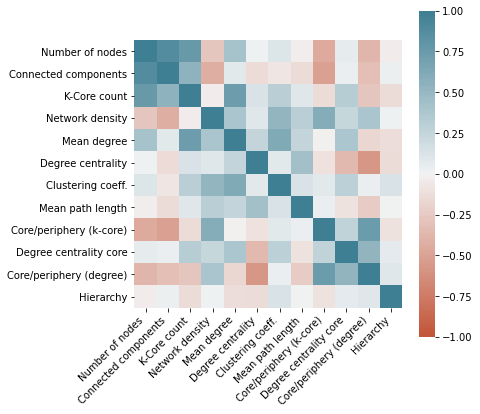
\includegraphics[width=0.7\textwidth]{figures/quantitative/corr_matrix/corr_before.png}
    \caption{Correlation matrix of release regularity, lines changed and the other collaboration metrics before the release.}
    \label{fig:corr_matrix}
\end{figure}

Based on these categories, the following correlation types can be seen:

\begin{itemize}
    \item \textbf{High positive linear correlation:} 
    \newline Number of nodes $\sim$ Connected components (0.88)
    \newline Number of nodes $\sim$ K-core count (0.76)
    \newline Core/periphery (k-core) $\sim$ Core/periphery (degree) (0.74)
    \newline Mean degree $\sim$ K-core count (0.73) 
    \item \textbf{Moderate positive linear correlation:}
    \newline Mean degree $\sim$ Clustering coefficient (0.61)
    \newline Network density $\sim$ Core/periphery (k-core) (0.59)
    \newline Connected components $\sim$ K-core count (0.54)
    \newline Degree centrality core $\sim$ Core/periphery (degree) (0.53)
    \newline Network density $\sim$ Clustering coefficient (0.52)
    \item \textbf{Low positive linear correlation:}
    \newline Degree centrality $\sim$ Mean path length (0.43)
    \newline Number of nodes $\sim$ Mean degree (0.41)
    \newline Network density $\sim$ Mean degree (0.39)
    \newline Network density $\sim$ Core/periphery (degree) (0.39)
    \newline Mean degree $\sim$ Degree centrality core (0.39)
    \newline K-core count $\sim$ Degree centrality core (0.33)
    \newline Clustering coefficient $\sim$ K-core count (0.31)
    \newline Network density $\sim$ Mean path length (0.30)
    \item \textbf{Low negative linear correlation:}
    \newline Number of nodes $\sim$ Core/periphery (k-core) (-0.46)
    \newline Network density $\sim$ Connected components (-0.44)
    \newline Number of nodes $\sim$ Core/periphery (degree) (-0.37)
    \newline Degree centrality $\sim$ Degree centrality core (-0.36)
    \newline Connected components $\sim$ Core/periphery (degree) (-0.32)
    \item \textbf{Moderate negative linear correlation:}
    \newline Degree centrality $\sim$ Core/periphery (degree) (-0.57)
    \newline Connected components $\sim$ Core/periphery (k-core) (-0.51)
\end{itemize}

From these significant correlations and based in Figure \ref{fig:corr_matrix} we can see that the number of nodes has one of the largest correlation with all the other variables. This proves that one of the greatest influence on the network metrics is the number of developers, and in extension, the activity within the repository. The k-core count, which measures the number of nodes having a degree number within the top 20th percentile, is highly positively correlated with the number of nodes, which indicates that the number of core developers in the network increases in proportion to the network size. However, the number of core developers classified by the degree centrality method does not indicate any relationship, which leads to the conclusion that these two methods do not identify the same collaborators as core members all the time, and there are significant differences. The low positive linear correlation between the two variables also confirms this observation.

The two derived core and periphery measures, however, are both negatively correlated with the number of nodes, indicating that as the network grows, the core becomes relatively smaller within the graph, meaning that most of the network growth can be contributed to the increased number of periphery developers. This observation is in line with the findings of McClean et al. \cite{mccleanSocialNetworkAnalysis2021}, who found that the number of core members tends not to change. The two core-periphery ratio metrics also show a high positive correlation, which shows that they both cover the same concept and measure the same property of the network.

\subsubsection{Network metrics hypotheses}

We theorize based on our observations so far that the larger the change is within the network, the larger the release is, and consequently, more lines are changed. We test this theory with an OLS linear regression for four chosen network metrics, which proved to be closely related to the collaboration network in any relation.

The \textbf{mean path length} shows what the average of the shortest distances between all pairs of developers in the network is. From an organizational point of perspective, this translates to how fast information can reach a developer from another developer in the best-case scenario (meaning always taking the shortest route) on average. Our theory is that during normal, 'business as usual' times, there is a core developer team, which is collaborating with all the periphery users, who are reporting bugs, suggesting new features, and helping in the development. This causes the mean path length to be relatively high between periphery members, as they are all connected to the core but not necessarily to each other. However, during the preparation of a (larger) release, the tasks shift from development to testing, reviewing, and integration, making developers more dependent on each other. 

\begin{quote}
    \textit{H2: There is less independence between developers at releases.}
\end{quote}

This could prompt the periphery members to interact with other periphery members, not directly just with the core, which ultimately lowers the mean path length before a release as less interdependence is required. After a release, we theorize that the focus shifts from development to planning, which again emphasizes the core developers and their activities, thus creating a more centralized structure and raising the mean path length.

Although mean path length indicates the shortest path for information to travel, which somewhat describes the level of collaboration as well, we use the \textbf{clustering coefficient} to measure the clusteredness of the network. The clustering coefficient is calculated by finding triangles within the graph: 'Is the neighbor of my neighbor also my neighbor?'. A high clustering coefficient indicates that a relatively large number of these triangles are present compared to all the triangles possible. From a project management perspective, a high clustering coefficient means strong group work and coordination, as the developers are clustered together, where most of them are connected to each other. We expect the clustering coefficients to rise before a release because the tasks shift from individual development to integration and regression testing, plus the coordination effort from the core members also increases, which promotes cross-checking tasks and reviewing each other's code. The clustering coefficient is expected to drop after a release, as activity becomes normal again when everyone is working on their own sections and functions.


\begin{quote}
    \textit{H3: Developers are clustered together significantly more during a release.}
\end{quote}


\textbf{Hierarchy}, as the third choice of metrics, considers both the clustering coefficient and the degree number by setting a trendline on a clustering coefficient-degree number plot and takes the slope of this trend. Hierarchy describes how strict the management roles are in the network. A node with a low clustering coefficient but a high degree number is likely to play an organizer or management role in the development process, as they are not collaborating on the source code as much as the other developers, but instead, they enable said developers by connecting them to other groups. In networks where there is a high hierarchy rate, the clustering coefficient decreases much faster by the increase of degree number, which results in a steeper declining trendline. Therefore, the lower the slope is, the more hierarchical the network is. Regarding the releases, due to the increase in activity before a release from all parties, our expectation is that the network gets less hierarchical due to the more cross-group collaboration, which causes the slope to rise. 

\begin{quote}
    \textit{H4: The developer network becomes less hierarchical during a release.}
\end{quote}

We expect the hierarchy to rise immediately after the release because the next development cycle needs to be planned, which requires organization and a highly structured breakdown of the backlog. Then later, it gets back to normal levels between two releases.

Lastly, we take the \textbf{core-periphery ratio} measure. This metric is a percentage of how many developers in the network are classified as core members compared to the overall number of nodes within it. We have two methods to classify a developer as a member of the core. The first is the K-core method, which is the number of nodes having at least $k$ degrees, and the second is the degree centrality core method, with which we calculate the degree centrality for each node. We consider a developer core for both methods if they are in the top 20th percentile of nodes. For both K-core and degree centrality core, the percentile is calculated starting from 0 and not from the lowest value within the network. This ensures that in time periods, when only the core is active, all the core members can still be identified as core since their absolute values are still high. Before a release, the core-periphery ratio is expected to fall because more periphery developers are being involved in the testing and integration tasks, but the number of core members stays the same during the project's lifecycle. This causes the ratio to fall as the overall number of nodes increase, but not the number of cores. After a release, this is expected to rise again due to the project focus shifting to planning and organizing, which involves more the core development team.

\begin{quote}
    \textit{H5: More periphery developers are involved at a release.}
\end{quote}

In order to confirm or reject the above hypotheses, we perform an Ordinary Least Squares (OLS) linear regression on the mentioned network statistics before and after a new release. We assume that the larger the network change is before and after the new version, the larger the release is. We use the following formula for this:

 \[ change \sim (m_2 - m_1) + N_1 + C(repo) \]

 where $m_1$ is the network metric value for one of the four chosen measures before the release, $m_2$ is directly after the release, $N_1$ is the number of nodes in the network before the release, and $C(repo)$ is the categorical value of the repository name as a dummy variable. The 'before' metric is calculated for the network generated from the period starting 28 days before and ending on the release day, and the 'after' value is calculated from the release day until 28 days past the release. We use the difference between the 'before' and 'after' values to represent the change. The number of nodes is also added in the regression to normalize the inherent differences that stem from the project's size.

 \begin{table}[!htbp] \centering
    \resizebox{\textwidth}{!}{%
    \begin{tabular}{@{\extracolsep{5pt}}lccccc}
    \\[-1.8ex]\hline
    \hline \\[-1.8ex]
    & \multicolumn{5}{c}{\textit{Dependent variable:}} \
    \cr \cline{5-6}
    \\[-1.8ex] & (1) & (2) & (3) & (4) & (5) \\
    \hline \\[-1.8ex]
     Clustering coeff & -0.18$^{}$ & & & & \\
      & (0.29) & & & & \\
     Core periphery degree & & & & -0.06$^{}$ & \\
      & & & & (0.19) & \\
     Core periphery k-core & & & & & 0.08$^{}$ \\
      & & & & & (0.26) \\
     Hierarchy & & & -0.29$^{}$ & & \\
      & & & (0.49) & & \\
     Mean path length & & 0.41$^{*}$ & & & \\
      & & (0.25) & & & \\
    \hline \\[-1.8ex]
     Observations & 4,078 & 4,078 & 4,078 & 4,078 & 4,078 \\
     $R^2$ & 0.31 & 0.31 & 0.31 & 0.31 & 0.31 \\
     Residual Std. Error & 0.29 & 0.25 & 0.49 & 0.19 & 0.26 \\
     F Statistic & 30.2$^{***}$ & 30.2$^{***}$ & 30.2$^{***}$ & 30.2$^{***}$ & 30.2$^{***}$ \\
     & (df = 61; 4016) & (df = 61; 4016) & (df = 61; 4016) & (df = 61; 4016) & (df = 61; 4016) \\
    \hline
    \hline \\[-1.8ex]
    \textit{Note:} & \multicolumn{5}{r}{$^{*}$p$<$0.1; $^{**}$p$<$0.05; $^{***}$p$<$0.01} \\
    \end{tabular}
    }
    \caption{The network statistics do not have a statistically significant influence on the \textbf{log} of the number of lines changed in the release.}
    \label{tab:size-metrics-log}
\end{table}


\begin{table}[!htbp] \centering
    \resizebox{\textwidth}{!}{%
    \begin{tabular}{@{\extracolsep{5pt}}lccccc}
    \\[-1.8ex]\hline
    \hline \\[-1.8ex]
    & \multicolumn{5}{c}{\textit{Dependent variable:}} \
    \cr \cline{5-6}
    \\[-1.8ex] & (1) & (2) & (3) & (4) & (5) \\
    \hline \\[-1.8ex]
     Clustering coeff & \num{4.2e+8}$^{**}$ & & & & \\
      & (\num{2.0e+8}) & & & & \\
     Core periphery degree & & & & \num{0.8e+8}$^{}$ & \\
      & & & & (\num{1.4e+8}) & \\
     Core periphery k-core & & & & & \num{-0.5e+8}$^{}$ \\
      & & & & & (\num{1.8e+8}) \\
     Hierarchy & & & \num{1.0e+8}$^{}$ & & \\
      & & & (\num{3.5e+8}) & & \\
     Mean path length & & \num{0.7e+8}$^{}$ & & & \\
      & & (\num{1.8e+8}) & & & \\
    \hline \\[-1.8ex]
     Observations & 4,078 & 4,078 & 4,078 & 4,078 & 4,078 \\
     $R^2$ & 0.07 & 0.07 & 0.07 & 0.07 & 0.07 \\
     Residual Std. Error & \num{2.0e+8} & \num{1.8e+8} & \num{3.5e+8} & \num{1.4e+8} & \num{1.8e+8} \\
     F Statistic & 5.1$^{***}$ & 5.1$^{***}$ & 5.1$^{***}$ & 5.1$^{***}$ & 5.1$^{***}$ \\
     & (df = 61; 4016) & (df = 61; 4016) & (df = 61; 4016) & (df = 61; 4016) & (df = 61; 4016) \\
    \hline
    \hline \\[-1.8ex]
    \textit{Note:} & \multicolumn{5}{r}{$^{*}$p$<$0.1; $^{**}$p$<$0.05; $^{***}$p$<$0.01} \\
    \end{tabular}
    }
    \caption{Only the clustering coefficient has a significance level of less than $0.05$ for explaining the number of lines changed in the new version.}
    \label{tab:size-metrics-normal}
\end{table}

The regression results are depicted in Table \ref{tab:size-metrics-log} and \ref{tab:size-metrics-normal}. We run the regressions for both the logarithm of the change size and the change size itself for all the metrics one by one, a total of 10 runs. With the alpha $\alpha = 0.05$ significance level, the only variable where $p < \alpha$ is the clustering coefficient in the normal, non-logarithmic change size regression with a value of $p = 0.04$. Based on this result, we can only reject the null hypothesis for the clustering coefficient, and we cannot reject it for the other metrics. Surprisingly the coefficient of the clustering coefficient is positive, which is contrary to our expectations. Our theory expected the clustering coefficient (CC) to rise before a release and drop afterward, which would result in a negative value when subtracting the 'before' value from the 'after' value. Therefore, in the regression model, the coefficient of CC would be negative, indicating an inverse relationship between the number of lines changed in the release and the CC change. Our findings, however, provide evidence for a positive linear relationship, which indicates that a unit of increase in the CC after the release corresponds to \num{4.2e+8} more lines changed in the release. Since the CC can only be between $0$ and $1$, we use $0.1$ as a base unit, which means that a $0.1$ increase in CC from before to after a new version causes the release to have \num{4.2e+7} more lines changed on average.

\subsubsection{Release size and issues opened and closed}

One explanation could be for the increase in clustering coefficient that a larger release with more lines changed leaves more room for errors and bugs within the code. The increase in issues leads to a higher bug fixing activity within the project, which requires cross-checking and integration tests, and ultimately causes more developer triangles to form, which raises the clustering coefficient value. To test this theory, we perform a similar OLS linear regression, but with two new metrics: number of issues opened and number of issues closed. If our assumptions are correct, there should also be a positive linear relationship between the release size measured in the number of lines changed, and the difference between the number of issues opened after and before the release. We also perform the regression for the number of issues closed. However, since the observed period after a new version is 28 days, but an issue might take longer than that on average to fix, we might not see the surge of new issues closed within this period.

\begin{quote}
    \textit{H6a: More issues opened before and after a release means more lines changed in the new version.}
\end{quote}

\begin{quote}
    \textit{H6b: More issues closed before and after a release means more lines changed in the new version.}
\end{quote}

Since the number of issues is not related to the collaboration network and are unrelated variables, we leave it out of the regression. Also, we use the values from before and after the release separately and without subtracting them from each other. The network metrics needed to consider the change between the 'before' and 'after' values because the change is measured from 0 on a scalar scale, but that is not necessarily the expected value in a network. On the other hand, the number of issues is0 by default, when no activity or issues are created.

Table \ref{tab:size-issues-log} and \ref{tab:size-issues} shows the OLS regression results for the number of issues opened and closed, both for 28 days before the release date and 28 days after it, respectively. We run the model for both the logarithm of the number of lines changed and the normal values separately. All four of our variables do not exceed the $\alpha = 0.05$ significance level for the $log$ of number of lines changed; however, this cannot be said for the number of lines changed without the logarithm, as none of them reach the required significance level.

\begin{table}[!htbp] \centering
    \resizebox{\textwidth}{!}{%
    \begin{tabular}{@{\extracolsep{5pt}}lcccc}
    \\[-1.8ex]\hline
    \hline \\[-1.8ex]
    & \multicolumn{4}{c}{\textit{Dependent variable:}} \
    \cr \cline{4-5}
    \\[-1.8ex] & (1) & (2) & (3) & (4) \\
    \hline \\[-1.8ex]
     Intercept & 19.567$^{***}$ & 19.582$^{***}$ & 19.567$^{***}$ & 19.567$^{***}$ \\
      & (3.873) & (3.873) & (3.872) & (3.873) \\
     Issues closed (log) $t_1$ & & & & -0.008$^{**}$ \\
      & & & & (0.003) \\
     Issues closed (log) $t_{-1}$ & & & -0.016$^{***}$ & \\
      & & & (0.005) & \\
     Issues opened (log) $t_1$ & & -0.007$^{**}$ & & \\
      & & (0.003) & & \\
     Issues opened (log) $t_{-1}$ & -0.007$^{**}$ & & & \\
      & (0.003) & & & \\
    \hline \\[-1.8ex]
     Observations & 5,216 & 5,216 & 5,216 & 5,216 \\
     $R^2$ & 0.267 & 0.267 & 0.268 & 0.267 \\
     Adjusted $R^2$ & 0.258 & 0.258 & 0.259 & 0.258 \\
     Residual Std. Error & 3.873(df = 5153) & 3.873(df = 5153) & 3.872(df = 5153) & 3.873(df = 5153)  \\
     F Statistic & 30.293$^{***}$ & 30.280$^{***}$ & 30.363$^{***}$  & 30.288$^{***}$  \\
     &  (df = 62; 5153) & (df = 62.0; 5153) & (df = 62; 5153) & (df = 62; 5153) \\
     \hline
    \hline \\[-1.8ex]
    \textit{Note:} & \multicolumn{4}{r}{$^{*}$p$<$0.1; $^{**}$p$<$0.05; $^{***}$p$<$0.01} \\
    \end{tabular}
    }
    \caption{The number of issues opened and closed both predict the $log$ of number of lines changed with a negative coefficient.}
    \label{tab:size-issues-log}
\end{table}

\begin{table}[!htbp] \centering
    \resizebox{\textwidth}{!}{%
    \begin{tabular}{@{\extracolsep{5pt}}lcccc}
    \\[-1.8ex]\hline
    \hline \\[-1.8ex]
    & \multicolumn{4}{c}{\textit{Dependent variable:}} \
    \cr \cline{4-5}
    \\[-1.8ex] & (1) & (2) & (3) & (4) \\
    \hline \\[-1.8ex]
     Intercept & \num{3.1e+8}$^{}$ & \num{3.2e+8}$^{}$ & \num{3.1e+8}$^{}$ & \num{3.1e+8}$^{}$ \\
      & (\num{2.5e+9}) & (\num{2.5e+9}) & (\num{2.5e+9}) & (\num{2.5e+9}) \\
     Issues closed $t_1$ & & & & \num{-2.5e+6}$^{}$ \\
      & & & & (\num{2.0e+6}) \\
     Issues closed $t_{-1}$ & & & \num{-4.9e+6}$^{}$ & \\
      & & & (\num{3.4e+6}) & \\
     Issues opened $t_1$ & & \num{-3.2e+6}$^{*}$ & & \\
      & & (\num{2.0e+6}) & & \\
     Issues opened $t_{-1}$ & \num{-2.0e+6}$^{}$ & & & \\
      & (\num{1.9e+6}) & & & \\
    \hline \\[-1.8ex]
     Observations & 5,216 & 5,216 & 5,216 & 5,216 \\
     $R^2$ & 0.075 & 0.075 & 0.075 & 0.075 \\
     Adjusted $R^2$ & 0.064 & 0.064 & 0.064 & 0.064 \\
     Residual Std. Error & \num{2.5e+9}(df = 5153) & \num{2.5e+9}(df = 5153) & \num{2.5e+9}(df = 5153) & \num{2.5e+9}(df = 5153)  \\
     F Statistic & 6.716$^{***}$ & 6.744$^{***}$  & 6.733$^{***}$ & 6.724$^{***}$ \\
      &  (df = 62.0; 5153.0) & (df = 62.0; 5153.0) & (df = 62.0; 5153.0) & (df = 62.0; 5153.0) \\
     \hline
    \hline \\[-1.8ex]
    \textit{Note:} & \multicolumn{4}{r}{$^{*}$p$<$0.1; $^{**}$p$<$0.05; $^{***}$p$<$0.01} \\
    \end{tabular}
    }
    \caption{The amount of lines changed also has a negative coefficient with the issues opened and closed, but the $p$ values are not significant.}
    \label{tab:size-issues}
\end{table}

Interestingly, there is a negative correlation between the number of lines changed and the number of issues closed and opened both before and after the release. Because we have seen that patch releases tend to have the lowest number of lines changed in the source code, by combining the results, we can see that the patch releases result in more issues closed. From a development point of perspective, this can be explained by the difference in handling a bug and a feature issue differently: By the definition of the semantic versioning system, a major and a minor release introduces new features to the software, whereas a patch mainly contains bugs. This creates an imbalance in the number of lines changed, as a completely new feature is likely to require more changes to the source code than a bug. Based on the data, it can be confirmed that major and minor releases have much more lines changed due to incorporating overwhelmingly feature and not bug issues, whereas patch releases resolve many bug issues with only a small number of lines changed. We separated the issues opened before and after into two variables, but since both of them are significant according to the model, we do not draw conclusions regarding specifically closing the issue before or after the new version. Mainly because we have seen previously that the time of close can be somewhat arbitrary: Some projects can follow a release plan, in which they close the issues resolved in the new version shortly before the release, or they can also wait for the release first and close the issues afterward in order to see the acceptance and reactions of the change (or just by pure administration purposes). 

\subsubsection{Normalizing the network metrics}

The linear regression models helped us understand how much the developer network changes at a new release compared to the release's size by contrasting the immediate period before and after the release. In this section, we investigate how the network metrics can be normalized.\\

Due to the inherent correlations between network size and the other metrics, such as clustering coefficient or average degree, we always need to ensure that the values being used are normalized or that the size difference between networks is controlled. This is why we used the Z-value in the qualitative analysis section (Section \ref{sec:patterns}), and this is also the reason why the network size was included in the regression models when the network metrics were used. The Z-value metrics provide a convenient and reliable way of eliminating the role of network size, as the actual network is being compared to many same-sized random networks. However, the Z-value generation only works when the network size is sufficiently large. As described in Section \ref{sec:density_degree}, the Z-value divides by the standard deviation of the random network's metric being calculated. In cases when the standard deviation is $0$, the Z-value cannot be interpreted, as this leads to a division by zero error. The standard deviation can only be $0$, if all values within the sample are precisely the same, and this scenario often plays out when the size of the network is small. As the size of the network becomes smaller and smaller, there are fewer variations to organize the $N$ nodes and $E$ edges, which raises the possibility of the random networks being repeated by generating the same network just by pure chance. Furthermore, when calculating the network metrics, the nodes and edges are not differentiated in any way: the metric will be the same, whether developer 'A' collaborates with developer 'B' or developer 'C'. This variability also increases the random networks having the same values for the measured metrics.

This phenomenon often occurs in our collection of repositories because there are a relatively low number of nodes within the networks generated immediately before or after a release (usually around 8-9). Therefore, most of the calculated Z-values cannot be interpreted. In order to correct for the disproportionality the network size can cause so that the graphs can be compared across all projects and sizes, we use an analytical approach to normalize the values. By dividing the theoretical maximum value of a metric in terms of its size, this is achievable.

The \textbf{mean path length} is calculated by averaging all the shortest path lengths between all pairs of developers. The theoretical maximum value of mean path length $l_G^*$ in terms of graph size is $l_G^* = (n-1)/2$ of network $G(N,E)$, where $|N| = n$ the number of nodes. Therefore, we calculate the normalized mean path length as follows:

\[ \hat{l}_G = \frac{2l_G}{n-1} \]

When it comes to the \textbf{clustering coefficient}, however, it is impacted differently by the size of the network because the CC is more or less independent of the number of nodes, and it is more related to the number of edges and the degree number. The clustering coefficient takes on its maximum value of $1$ only in complete graphs, as the number of triangles within the graph is at maximum when every node is connected to all other nodes. Therefore, we normalize the CC values with the formula used by Gentner et al. \cite{gentnerLargeValuesClustering2016} for the maximum clustering coefficient of a $k$-regular connected graph:

\[ \hat{C}(G) = \frac{C(G)}{(1-\frac{6}{k(k+1)})}\]

where $k$ is the degree number of nodes in a $k$-regular graph. \\

The \textbf{core-periphery ratio} already takes into account the number of nodes, which is a proxy for the network size, as the CP-ratio is calculated by dividing the number of nodes in the top 20th percentile of either degree centrality or k-cores, and then dividing by the overall number of nodes, meaning there is no need for normalization.

\textbf{Hierarchy} is more complex than the rest of the metrics, as it uses the combination of clustering coefficient and degree number to plot a scatter plot, and the slope of the linear trendline is used as the hierarchy value. By having more nodes in the graph, the trendline does not necessarily change, and it stays the same if the level of hierarchy does not change. For example, if a new team of developers appears in the network, who have a team leader just as all other teams, then the overall hierarchy of the network did not change, as managers still have the same number of developers under them in the organizational hierarchy. In contrast, if more people join the already available developer teams, a team leader will have more developers to manage, which causes the network to become less hierarchical. As we demonstrated, a network can grow in a manner that changes the hierarchy or independent of it, and therefore we conclude that there is no need for normalizing the hierarchy metric.

\subsubsection{Network measure trends}

After applying the normalization described above on our dataset, box plots are created to show the overall trend in measures at a release. However, this requires gathering and calculating metrics for more than two time periods (before and after a release) to represent the changes over time. In order to make the plots more straightforward, we shift the time window so that the chosen day is not at the beginning but in the middle of the observation period. This is depicted in Figure \ref{fig:time-window}, where the numbers on the timeline represent the number of weeks passed relative to the release day.

\begin{figure}[!htbp]
    \centering
    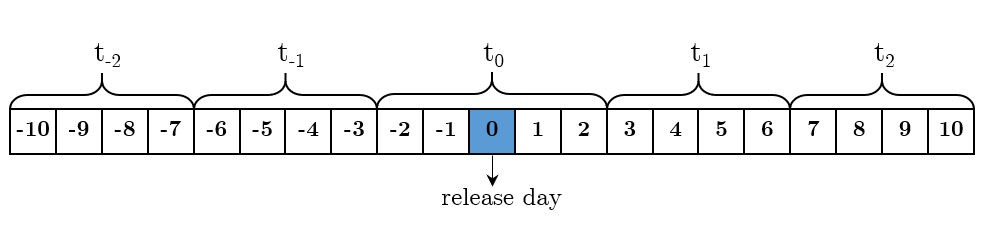
\includegraphics[width=\textwidth]{figures/quantitative/time_window.png}
    \caption{Time windows in weeks and their respective variable names.}
    \label{fig:time-window}
\end{figure}


Each metric's normalized value is calculated for each release's corresponding five timespans (from $t_{-2}$ to $t_2$). With this approach, another issue arises: releases, which were within two months of the data collection, will only have partial data available for the last three timespans. This can skew the results since for these values, the results will be 0, and it would falsely show a decline in activities. Therefore, we filter out those releases, which were created after \textit{1 January 2021}.

The results for \textbf{mean path length} can be seen in Figure \ref{fig:box-mean-path}. Contrary to our expectations, we see an increase in mean path length up until the release and a sharp decrease afterward. A decrease in mean path length means less interdependency among developers, as fewer people are fulfilling the 'middle man' role within the network, which was expected at a release since closer collaboration is required and different tasks, therefore developers have to move out of their usual role and collaborate with those, whom they do not often collaborate with. The reverse in the results suggests that the activity level is not as high as expected at a release. The likely reason is that not many changes are approved around the releases, and the focus is on finishing up the current tasks. Before, the shorter mean path length can be explained with the rush to finish the tasks, and after, it can be explained with the bug reports and new issues, and consequently their activity from the developers' side.

\begin{figure}[!htbp]
    \centering
    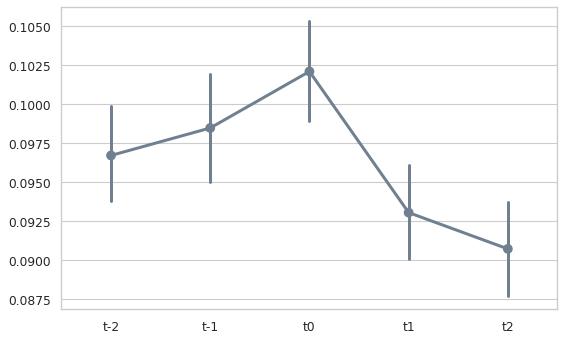
\includegraphics[width=\textwidth]{figures/quantitative/pointplots/mean_path_length.png}
    \caption{Normalized mean path length reaches its maximum at a release, and then sharply falls below usual.}
    \label{fig:box-mean-path}
\end{figure}

Because of the heterogeneity of each project, there could be considerable differences and patterns different from the one described above. Therefore, we plot each repository's mean path length boxplot separately, which are depicted in Appendix \ref{app:mean_path-box-app}. We exclude repositories that have less than ten observed releases before \texttt{1 January 2021} because that would reduce the number of releases aggregated on the plot, and the unique traits of the single particular releases would show.

After observing the total $53$ plots, we identify four main reoccurring patterns that can be observed within the projects. We name these patterns based on the two half-curves' steepness that would connect the five boxes depicted. These are:

\begin{itemize}
    \item \textit{Flat (11)}: Repositories following this pattern barely change at all, and their mean path length stays the same in all five timespans regardless of the release.
    \item \textit{Rise-decline (11)}: Projects falling into this category mainly follow the overall pattern depicted in Figure \ref{fig:box-mean-path}, which shows a rise until the release, then a decline afterward.
    \item \textit{Flat-decline (6)}: These projects stay flat until the release, but after the release, their mean path length drops.
    \item \textit{Decline-rise (6)}: Repositories following this pattern show the opposite observation than the aggregated view; that is, their metric declines until the release date, then it rises again.
\end{itemize}

\begin{figure}[!htbp]
    \centering
    \begin{subfigure}{0.49\textwidth}
        \centering
        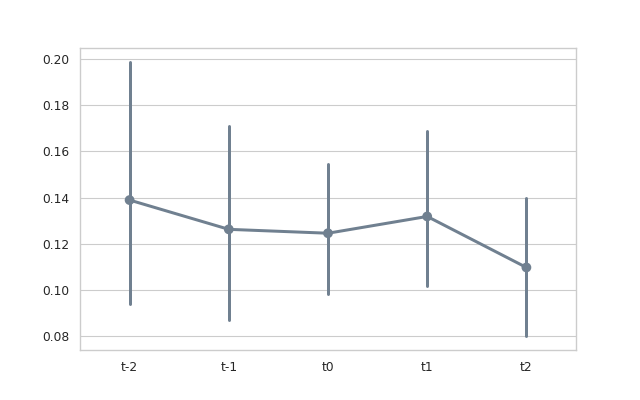
\includegraphics[width=\textwidth]{figures/quantitative/pointplots/nunit_nunit.png}
        \caption{Flat (\textit{nunit/nunit})}
        \label{fig:mean-path-pattern1}
    \end{subfigure}
    \begin{subfigure}{0.49\textwidth}
        \centering
        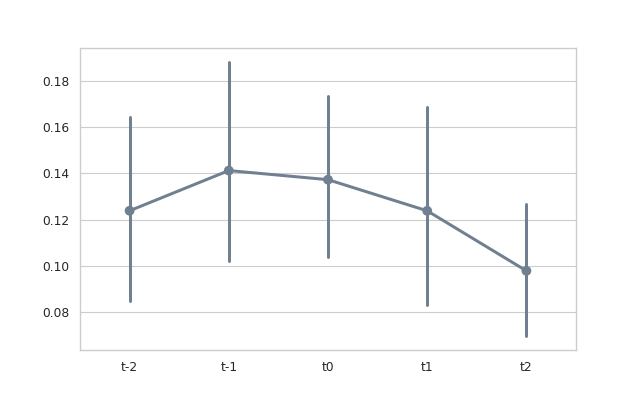
\includegraphics[width=\textwidth]{figures/quantitative/pointplots/stack-of-tasks_pinocchio.png}
        \caption{Rise-decline (\textit{fioprotocol/fio})}
        \label{fig:mean-path-pattern2}
    \end{subfigure}
    \begin{subfigure}{0.49\textwidth}
        \centering
        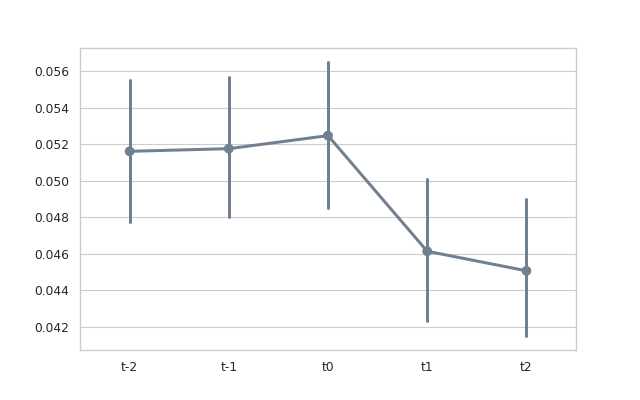
\includegraphics[width=\textwidth]{figures/quantitative/pointplots/frappe_erpnext.png}
        \caption{Flat-decline (\textit{frappe/erpnext})}
        \label{fig:mean-path-pattern3}
    \end{subfigure}
    \begin{subfigure}{0.49\textwidth}
        \centering
        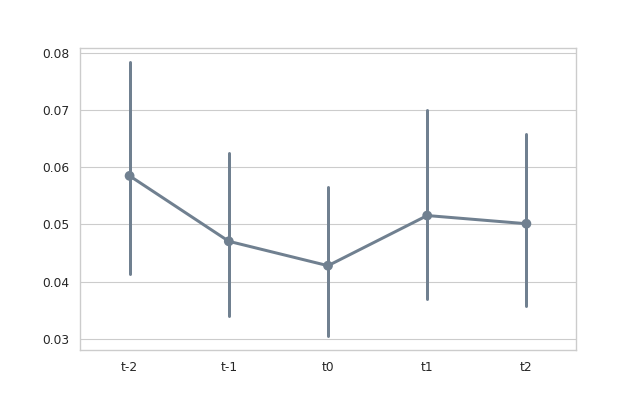
\includegraphics[width=\textwidth]{figures/quantitative/pointplots/swaywm_sway.png}
        \caption{Decline-rise (\textit{swaywm/sway})}
        \label{fig:mean-path-pattern4}
    \end{subfigure}
    \caption{The four observed patterns for mean path length.}
    \label{fig:box-mean-path-patterns}
\end{figure}

Examples for all four categories are shown in Figure \ref{fig:box-mean-path-patterns}. The first, flat type can be easily interpreted: in some projects, there is no relation between release and mean path length, and the distance between developers is the same all along the project lifecycle. The rise-decline pattern can be explained with the network getting bigger or with the absence of core members at a release, lengthening the average distance between developers. Therefore, the opposite, decline-rise pattern is an example of the heavier involvement of the core, which also connects to more periphery due to their increased activity and organizational tasks. Finally, the flat-decline pattern suggests that some projects can be unaffected by the preparation for a new version, and they are only affected at the later timespans when the core is more involved (as explained before).

\begin{figure}[!htbp]
    \centering
    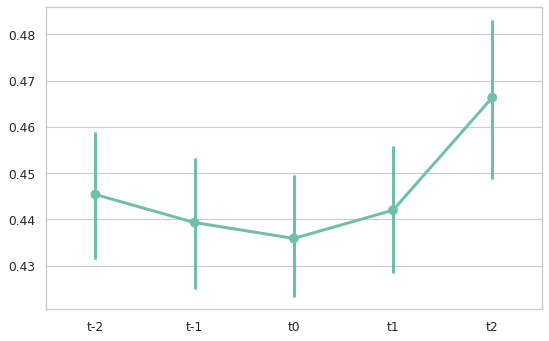
\includegraphics[width=\textwidth]{figures/quantitative/pointplots/clustering_coeff_filtered.png}
    \caption{Clustering coefficient release trend after the removal of 0 values.}
    \label{fig:clustering-box}
\end{figure}

We also performed the same analysis on the \textbf{normalized clustering coefficient}; however, the results are inconclusive, as the majority of all release's normalized clustering coefficient is $0$. Therefore, we removed the releases from the plot data, which had at least one CC value equal to $0$. The resulting box plot (shown in Figure \ref{fig:clustering-box}) follows a \textit{flat-rise} pattern, which is especially visible at timespan $t2$, where the box is significantly higher than the other periods. However, the removal of 0-values reduced below 10\% the number of releases included in the observation; therefore, we cannot conclude anything definitive regarding the clustering coefficient. For all repositories separately, the clustering coefficient point plots can be seen in Appendix \ref{app:boxplots}. \\

The same method is used to visualize the \textbf{number of issues opened and closed} for the releases. This is depicted in Figure \ref{fig:issues-box}. We can see a clear increase in both issues opened and issues closed. The number of issues opened shows a steady and constant increase for all five timespans, which can mean that the rate at which new issues are opened tends to increase in general within a project over time. If the issues opened slowly increases over time regardless of other events, such as a new release, then naturally, the $t_2$ timespan will show a slight increase in opened issues compared to the $t_{-2}$ since it always takes into account a time period five months later, and by that time the issue rate could have changed. In order to attribute the increase in the number of issues opened, we would need to see a sharp change at $t_0$ to rule out the option of the steady increase.

\begin{figure}[!htbp]
    \centering
    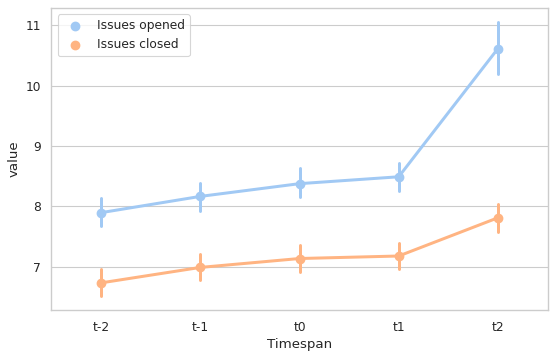
\includegraphics[width=\textwidth]{figures/quantitative/pointplots/issues.png}
    \caption{The issue activities are higher after a release than before, but at all times, there are more issues opened than closed.}
    \label{fig:issues-box}
\end{figure}

The number of issues closed, on the other hand, shows a much more sudden change. Up until, and including the timespan containing the release day, the average stays zero, but after the release, in $t_1$ and $t_2$ we see a sharp rise. This indicates that a new version and the number of issues closed are related. The issues being closed are likely to be those features and bugs that were implemented and distributed with the new release. Therefore, we can say that most projects manage the issues by first implementing and deploying it, and only then closing it. Otherwise, we would see the sharp increase before the release timespan and not after it. \\

Just with the other metrics, the \textbf{core-periphery ratio} is also heavily dependent on the unique properties of the observed repositories, which is also the cause why the box plot of all projects aggregated does not show any change, regardless of the timespans. On further investigation, we found that a significant number (16) of repositories have the box plots 'stuck' to the maximum value $1$. This is attributed to the very low number of nodes in the generated networks: when there are only 2 or 3 developers in the network, their degree centralities are more likely to be in the top 20th percentile starting from zero. We remove these projects from the aggregation not to obscure the trends of the other repositories with a more extended developer network and depict their box plot for the degree centralization core-periphery ratio in Figure \ref{fig:cp-box}.

\begin{figure}[!htbp]
    \centering
    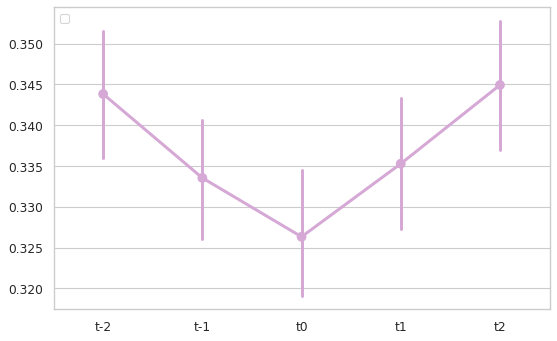
\includegraphics[width=\textwidth]{figures/quantitative/pointplots/cp_ratio.png}
    \caption{The core/periphery ratio shows a U-shape, where the minimum is reached at a release, showing that the DCN becomes significantly less clustered around that time.}
    \label{fig:cp-box}
\end{figure}

With the remaining 45 repositories in aggregation, a slight V-shaped trend can be observed. This behavior is according to our theory and expectations, as they were expected to fall at the time of release due to the increased involvement of the periphery developers, which lowers the ratio of the core members within the network. However, when we look at the individual projects, just with the mean path length, we can also observe several trends within the repositories, followed by a subset of them. These trends are shown in Figure \ref{fig:cp-box-grid}, where one line of plots represents an observed trend, and the selected repository box plots shown in that line belong to that category. Not all repositories are depicted in the plot. The four trends in order from top to bottom are:

\begin{itemize}
    \item \textit{Rising}: A continuous rise from $t_{-2}$ to $t_2$ without any significant change at the release $t_0$.
    \item \textit{Falling}: The opposite of rising, as the core/periphery ratio continuously decreases over the five periods.
    \item \textit{Parabola}: The box plots draw a parabola or V-shape during the five timespans, where at the release $t_0$ it reaches its minimum, and then increases again to the 'normal' level. This is the most dominant pattern within the dataset, as this pattern is also observed in the aggregate boxplot, and also because this shape is seen in more of the plots than other trends.
    \item \textit{Wave}: These repositories show a wave form with the boxplots, as they start on a normal level, then there is a significant increase in $t_{-1}$, a continued decrease until $t_1$ and then a slight increase to reach the normal level again at $t_2$.
\end{itemize}

\begin{figure}[!htbp]
    \centering
    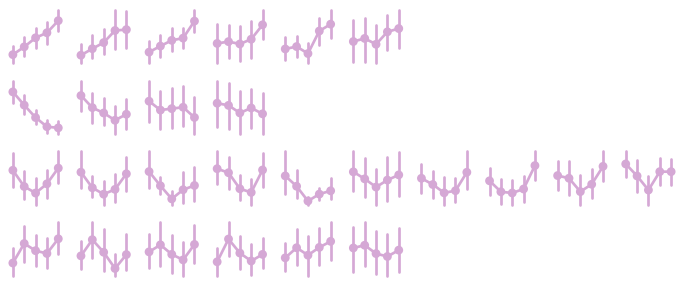
\includegraphics[width=\textwidth]{figures/quantitative/pointplots/cp_ratio_trends.png}
    \caption{The four observable core/periphery trends (rising, falling, parabola and wave), showing the most popular parabola as the most numerous, which causes the overall C/P to also take this form.}
    \label{fig:cp-box-grid}
\end{figure}


There could be several organizational reasons why these patterns exist. The obvious reason for the rising trend in the core-periphery ratio could be the rush before the release to include as much change as possible before it is released. This increase in activity involves more non-core developers, which keeps the ratio low before the release. However, after the new version is available, the focus shifts from development to planning, generating more core involvement than from the periphery developers, which raises the ratio value. The opposite, falling pattern could indicate the opposite effect: before the release, the development team might announce a 'code-freeze,' which prohibits the change of code before the release (or rather merging it into the release candidate). Since only authorized developers can change the release candidate, who are most likely core members, the cp ratio gets high. After the release, the sidelined changes are included, and the bug fixing period starts, which requires collaboration effort from not just the core developers, therefore the ratio decreases. The wave pattern could be the same effect as in the falling case, just happening in a much shorter period of time, which causes the outermost timespans to show the normal ratio level already. \\

\begin{figure}[!htbp]
    \centering
    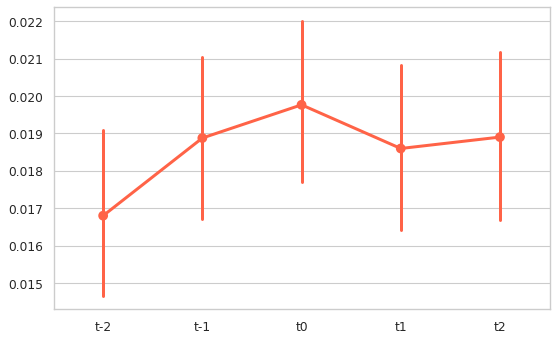
\includegraphics[width=\textwidth]{figures/quantitative/pointplots/hierarchy.png}
    \caption{The hierarchy tends to take on the highest values (the lowest hierarchy in the network) at a release, and stays relatively high after it.}
    \label{fig:hierarchy-box}
\end{figure}

Lastly, we take a look at the \textbf{hierarchy} boxplots in Figure \ref{fig:hierarchy-box}. The hierarchy is getting more widely distributed towards the positive values as we approach the release date, then the reversal can be seen. Although the change is rather small, it is still significant, as it follows a regular pattern. We can also see that the distribution is heavily skewed towards $0$ in all boxes, which indicates that the majority of values are $0$. Hierarchy takes on the value $0$ when the linear trendline is parallel to the X-axis on the scatter plot of degrees-CC, which is interpreted as the network being decentralized without any hierarchy. As we have discussed before, negative values mean a hierarchy exists in the network. Here we see positive values, which we can interpret as the increase of central hubs (developers) in the network. 

The trend towards the positive values describes a positive correlation between the degree number and the clustering coefficient, which signals that the developers connecting different segments of the DCN are also clustered with each other. Therefore, these developers comprise the core developer team, who do not exhibit any hierarchical properties and are connected directly to each other and loosely to the periphery developers during the release. This is directly opposite to our hypothesis: An increasingly hierarchical network was theorized due to the increased centralization and required approvals and planning. Here we confirm the opposite, as the network gets more 'chaotic' at the release and less organized than during the regular development periods.

\section{Discussion and results}

In Section \ref{sec:gitminer}, we propose a theoretical framework for analyzing developer collaboration networks (DCNs) in open-source projects, which we also implement using the \texttt{git2net} and \texttt{repo\_tools} mining libraries. After discussing the properties of temporal and static networks and describing the relevant network statistics, we implement a Python-based solution for the framework to find an answer to our research question.

By examining closely the change in network statistics in a selected group of projects in Section \ref{sec:patterns}, we observed how a new version's release changes the collaboration network's structure. We discovered some commonly occurring patterns in most projects, such as the network becoming highly non-hierarchical at a layoff event. The main realization was how different each project can behave and how uniquely they behave. As an example, the clustering coefficient proved to be a somewhat good predictor of a release in \texttt{pandas}, but the most significant change was expected at its only major release, where we could not observe any significant change. Whereas the \texttt{NetworkX} library has a spike perfectly coinciding with a new minor release, but other minor releases do not show any change. We also saw the release regularity to differ between repositories wildly: Some projects have an ad-hoc schedule, while others keep a very short or very long release cycle. However, we could observe the smaller projects following an ad-hoc schedule, signaling a lower level of organization.

The issue management also differs within each project, as each follows a different categorization scheme, and the maintenance also shows significant differences: Some projects close the issues before the release, some perform this afterward. The common trend between projects is the ever-increasing number of open issues.

To come to a general conclusion on what trends are applicable for the majority of OSS projects, we looked at a large number of randomly selected repositories in order to generalize how the developer network properties change on average in Section \ref{sec:quantitative}. After mining the selected repositories and discarding the not minable and badly versioned projects, we were left with 68 repositories with a diverse range of used languages, sizes, and release cycles. Based on our observations in Section \ref{sec:patterns}, we set eight hypotheses regarding the behavior of the DCN at a new release. A summary of these, along with the results, can be found in Table \ref{tab:hypothesis-results}. 

\begin{table}[!htbp]
    \centering
    \resizebox{\textwidth}{!}{%
        \begin{tabular}{|l|p{5cm}|l|l|}
            \hline
            \textbf{\#} & \textbf{Hypothesis}  & \textbf{Variable} & \textbf{Result} \\
            \hline
            $H_{1a}$ & A minor release has more lines changed than a patch release. & lines changed & Supported \\
            \hline
            $H_{1b}$ & A major release has more lines changed than a minor release. & lines changed & Not supported \\
            \hline
            $H_2$ & There is less independence between developers at releases. & mean path length & Reverse supported \\
            \hline
            $H_3$ & Developers are clustered together significantly more during a release. & clustering coefficient & Not supported \\
            \hline
            $H_4$ & The developer network becomes less hierarchical during a release & hierarchy & Supported \\
            \hline
            $H_5$ & More periphery developers are involved at a release. & core/periphery ratio & Supported \\
            \hline
            $H_{6a}$ &  More issues opened before and after a release means more lines changed in the new version. & issues opened & Reverse supported \\
            \hline
            $H_{6b}$ &  More issues closed before and after a release means more lines changed in the new version. & issues opened & Reverse supported \\
            \hline

        \end{tabular}
    }
    \caption{Summary of the hypotheses results.}
    \label{tab:hypothesis-results}
\end{table}

Regarding $H_{1a}$ and $H_{1b}$, we could only partially prove the positive relation between the semantic version number and the volume of source code change. While we proved that both minor and major releases contain more source code line changes than a patch release ($H_{1a}$ supported), we could not prove that a major release is also more significant in terms of lines than a minor release ($H_{1b}$ rejected). We contributed the latter result partially to the ambiguous version naming, such as parallel support for multiple major versions and the problem of how to classify \textit{beta} and \textit{rc} versions.

However, the rejection of $H_{1b}$ is consistent with the findings of $H_{6a}$ and $H_{6b}$. Contrary to our expectations, the number of issues closed and opened, both before and after a release negatively, and not positively correlate with the magnitude of the semantic version number. This implies that a major release does not lead to as many changes in issues as a patch, thereby proving that most tickets and issues are opened and closed with patch releases. Combined with $H_{1b}$, we can reasonably propose that major releases mainly focus on new, experimental features.

Considering the collaboration network structure at releases, we are also presented with mixed results. On the one hand, we could find substantial evidence for the increased involvement of the periphery developers within a project ($H_5$). Their theorized role is to help out in the preparation tasks, such as regression testing, but they could also be rushing to add changes to the source code so that their modifications are also included in the new version.

The sudden involvement of a larger number of contributors obscures the typical network structure of the central core and some active but casual developers. This is confirmed in $H_4$ by analyzing the hierarchy values over time. The networks' usual higher hierarchical construct becomes less organized as a large number of periphery developers are connected, and the hierarchy value rises (there is an inverse relation between hierarchy value and network hierarchy). This effect is emphasized even more due to the fact that the types of tasks also change during this period of time, which requires interaction with other community members who do not have to collaborate as often.

The observation and the conclusions we could draw from the clustering coefficient could tell which effect is more prominent: If the different tasks, and as a result the closer collaboration with community members further away in the organizational hierarchy, has a more significant impact on the hierarchy, the clustering coefficient would also show an increase at releases. On the other hand, a decrease or no change in the clustering coefficient, combined with an increase in non-hierarchical network structure, would suggest a more randomized network, where the nodes' clustering coefficient stays relatively the same due to the periphery developers connecting randomly to the established core members. However, we could not test these theories, as the method for normalizing the global clustering coefficient for the network's size did not provide a sufficiently stable output that could be aggregated across projects ($H_3$). 

The findings for $H_2$ supports the latter option: we found that contrary to our theory, the average shortest path between nodes increases at a release. This confirms that the majority of periphery developers showing an increased activity are not fulfilling a 'bridge' role between two developers but rather connect to the network randomly. This ultimately increases the network size, which raises the mean path length even when we normalize for the network growth.

All the data mining results\footnote{Data mining databases: \url{https://doi.org/10.5281/zenodo.5002638}} as well as the Python libraries, notebooks, and scripts\footnote{Python resources: \url{https://github.com/csepanyij/master-thesis}} can be found at the respective links in the footnote.

\section{Conclusion and future work}

In conclusion, we have seen how different each open-source project can be in the main programming language, size, release frequency, release regularity, versioning, hierarchy, and issue tracking, to name a few aspects. These differences make it difficult to draw a general conclusion about OSS projects, which is applicable to most repositories. Nevertheless, we have found some general observations regarding projects at releases, but these findings may not apply to all projects due to their uniqueness.

We could confirm the previous finding, which observed that semantic versioning is used inconsistently, because we found that contrary to the expectations, a major release is not larger than a minor release. A lack of consistent practices across different OSS projects can also be seen in the different release regularities: within our analysis we discovered, that some projects follow a seemingly random release schedule, while others implement a more regular planning of releases. An irregular schedule might be followed on a need basis, when the software's new version is announced after a certain number of new features are added. We have seen that this practice is mainly followed by smaller projects with fewer contributors, as there are fewer features and bug fixes implemented within a given timeframe. On the other hand, larger projects tend to have a more regular release cycle, where they collect the features added so far and bundle them in a new release regularly. The shortest of these plans was 2 months, and a 6-month cycle proved to be the most popular within our sample in Section \ref{sec:patterns}.

When we revisit our research questions asked in Section \ref{sec:motivation-rq}, we can answer \textit{RQ1} with a definitive yes: the foreseeable events, such as a new release, do change the collaboration structure. With the increased involvement of the periphery collaborators and a lower hierarchy, the network becomes more chaotic, even though the release date in most projects is known well before the release to most collaborators. The unsettled network is even worsened by the change in the types of tasks, such as more issue administration or testing tasks. However, despite the transformation of DCN due to a release, we have also seen that most projects reorganize themselves into their regular structure, meaning these changes are only temporary and the onion model stays stable on the long run. This is confirmed by the regularity of releases, as larger projects are able to maintain a regular release cycle.

The most prominent change the DCN goes through at a release is the increased involvement of periphery co-developers besides the core. We found evidence for this with the uptick of the mean path length in Figure \ref{fig:box-mean-path}, indicating the network becoming larger and longer paths are needed to reach individual developers. The rise in periphery activity is also visible in the core/periphery ratio on Figure \ref{fig:cp-box}, as the core's ratio compared to all developers shrinks, which further supports the larger non-core activity within the network.

Regarding \textit{RQ2}, we also have some notable findings regarding layoff events, where we have seen that the disappearance of the core developer network creates a highly disorganized network, and the hierarchy disappears. However, we could only confirm this finding with a few repositories, as we could not find an efficient way to reliably gather unexpected events within FLOSS projects, which is a limitation of our paper.

Therefore, we suggest performing the same network measures and observations on a list of repositories, where unexpected events are recorded, and their exact date is known. Also, specific events, such as the layoff of the core supporting team, can have fatal consequences regarding the project's outcome and success. We propose further research into how success can be measured within OSS projects based on factors like popularity, number of commits, contributors, and visitors. Furthermore, how the organizational measures and metrics discussed in this paper could affect the success or failure of the project.

Our findings show the number of issues created rise after a new release in Figure \ref{fig:issues-box}, which is a preliminary confirmation of new features introducing new bugs post-release. However, it is unknown how many of these are bugs and how many are new feature requests inspired by the publicity of the new version. Further studies could look into in which cases there are relatively more new bugs reported after a release, and how this is influenced by the change size of the new version that can be measured with the same methods displayed in this thesis.

As repositories become larger and more popular over time, we have found that a regular release cycle is adopted. This theorizes an existence of a maturity model, where there are potentially different stages of organizational maturity. Future research could also be conducted to discover these distinct levels and properties, which could ultimately be linked to the project's success.

Lastly, our simple issue classification method could only succeed for a tiny percentage of issues due to time limitations and the complexity of different projects' tagging methods. We propose a classifying tool that uses keywords and sentiment analysis, and text mining tools on various fields of a ticket to more precisely identify the bug and feature issues.